\documentclass[1p]{elsarticle_modified}
%\bibliographystyle{elsarticle-num}

%\usepackage[colorlinks]{hyperref}
%\usepackage{abbrmath_seonhwa} %\Abb, \Ascr, \Acal ,\Abf, \Afrak
\usepackage{amsfonts}
\usepackage{amssymb}
\usepackage{amsmath}
\usepackage{amsthm}
\usepackage{scalefnt}
\usepackage{amsbsy}
\usepackage{kotex}
\usepackage{caption}
\usepackage{subfig}
\usepackage{color}
\usepackage{graphicx}
\usepackage{xcolor} %% white, black, red, green, blue, cyan, magenta, yellow
\usepackage{float}
\usepackage{setspace}
\usepackage{hyperref}

\usepackage{tikz}
\usetikzlibrary{arrows}

\usepackage{multirow}
\usepackage{array} % fixed length table
\usepackage{hhline}

%%%%%%%%%%%%%%%%%%%%%
\makeatletter
\renewcommand*\env@matrix[1][\arraystretch]{%
	\edef\arraystretch{#1}%
	\hskip -\arraycolsep
	\let\@ifnextchar\new@ifnextchar
	\array{*\c@MaxMatrixCols c}}
\makeatother %https://tex.stackexchange.com/questions/14071/how-can-i-increase-the-line-spacing-in-a-matrix
%%%%%%%%%%%%%%%

\usepackage[normalem]{ulem}

\newcommand{\msout}[1]{\ifmmode\text{\sout{\ensuremath{#1}}}\else\sout{#1}\fi}
%SOURCE: \msout is \stkout macro in https://tex.stackexchange.com/questions/20609/strikeout-in-math-mode

\newcommand{\cancel}[1]{
	\ifmmode
	{\color{red}\msout{#1}}
	\else
	{\color{red}\sout{#1}}
	\fi
}

\newcommand{\add}[1]{
	{\color{blue}\uwave{#1}}
}

\newcommand{\replace}[2]{
	\ifmmode
	{\color{red}\msout{#1}}{\color{blue}\uwave{#2}}
	\else
	{\color{red}\sout{#1}}{\color{blue}\uwave{#2}}
	\fi
}

\newcommand{\Sol}{\mathcal{S}} %segment
\newcommand{\D}{D} %diagram
\newcommand{\A}{\mathcal{A}} %arc


%%%%%%%%%%%%%%%%%%%%%%%%%%%%%5 test

\def\sl{\operatorname{\textup{SL}}(2,\Cbb)}
\def\psl{\operatorname{\textup{PSL}}(2,\Cbb)}
\def\quan{\mkern 1mu \triangleright \mkern 1mu}

\theoremstyle{definition}
\newtheorem{thm}{Theorem}[section]
\newtheorem{prop}[thm]{Proposition}
\newtheorem{lem}[thm]{Lemma}
\newtheorem{ques}[thm]{Question}
\newtheorem{cor}[thm]{Corollary}
\newtheorem{defn}[thm]{Definition}
\newtheorem{exam}[thm]{Example}
\newtheorem{rmk}[thm]{Remark}
\newtheorem{alg}[thm]{Algorithm}

\newcommand{\I}{\sqrt{-1}}
\begin{document}

%\begin{frontmatter}
%
%\title{Boundary parabolic representations of knots up to 8 crossings}
%
%%% Group authors per affiliation:
%\author{Yunhi Cho} 
%\address{Department of Mathematics, University of Seoul, Seoul, Korea}
%\ead{yhcho@uos.ac.kr}
%
%
%\author{Seonhwa Kim} %\fnref{s_kim}}
%\address{Center for Geometry and Physics, Institute for Basic Science, Pohang, 37673, Korea}
%\ead{ryeona17@ibs.re.kr}
%
%\author{Hyuk Kim}
%\address{Department of Mathematical Sciences, Seoul National University, Seoul 08826, Korea}
%\ead{hyukkim@snu.ac.kr}
%
%\author{Seokbeom Yoon}
%\address{Department of Mathematical Sciences, Seoul National University, Seoul, 08826,  Korea}
%\ead{sbyoon15@snu.ac.kr}
%
%\begin{abstract}
%We find all boundary parabolic representation of knots up to 8 crossings.
%
%\end{abstract}
%\begin{keyword}
%    \MSC[2010] 57M25 
%\end{keyword}
%
%\end{frontmatter}

%\linenumbers
%\tableofcontents
%
\newcommand\colored[1]{\textcolor{white}{\rule[-0.35ex]{0.8em}{1.4ex}}\kern-0.8em\color{red} #1}%
%\newcommand\colored[1]{\textcolor{white}{ #1}\kern-2.17ex	\textcolor{white}{ #1}\kern-1.81ex	\textcolor{white}{ #1}\kern-2.15ex\color{red}#1	}

{\Large $\underline{12a_{0346}~(K12a_{0346})}$}

\setlength{\tabcolsep}{10pt}
\renewcommand{\arraystretch}{1.6}
\vspace{1cm}\begin{tabular}{m{100pt}>{\centering\arraybackslash}m{274pt}}
\multirow{5}{120pt}{
	\centering
	\includegraphics[width=112pt]{../../../GIT/diagram.site/Diagrams/png/1147_12a_0346.png}\\
\ \ \ A knot diagram\footnotemark}&
\allowdisplaybreaks
\textbf{Linearized knot diagam} \\
\cline{2-2}
 &
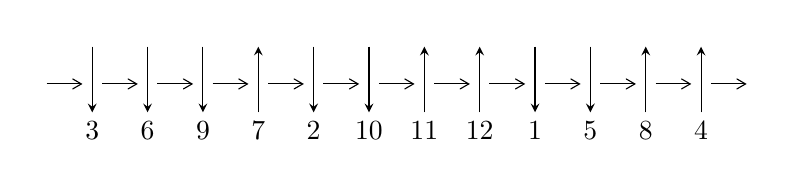
\begin{tikzpicture}[x=20pt, y=17pt]
	% nodes
	\node (C0) at (0, 0) {};
	\node (C1) at (1, 0) {};
	\node (C1U) at (1, +1) {};
	\node (C1D) at (1, -1) {3};

	\node (C2) at (2, 0) {};
	\node (C2U) at (2, +1) {};
	\node (C2D) at (2, -1) {6};

	\node (C3) at (3, 0) {};
	\node (C3U) at (3, +1) {};
	\node (C3D) at (3, -1) {9};

	\node (C4) at (4, 0) {};
	\node (C4U) at (4, +1) {};
	\node (C4D) at (4, -1) {7};

	\node (C5) at (5, 0) {};
	\node (C5U) at (5, +1) {};
	\node (C5D) at (5, -1) {2};

	\node (C6) at (6, 0) {};
	\node (C6U) at (6, +1) {};
	\node (C6D) at (6, -1) {10};

	\node (C7) at (7, 0) {};
	\node (C7U) at (7, +1) {};
	\node (C7D) at (7, -1) {11};

	\node (C8) at (8, 0) {};
	\node (C8U) at (8, +1) {};
	\node (C8D) at (8, -1) {12};

	\node (C9) at (9, 0) {};
	\node (C9U) at (9, +1) {};
	\node (C9D) at (9, -1) {1};

	\node (C10) at (10, 0) {};
	\node (C10U) at (10, +1) {};
	\node (C10D) at (10, -1) {5};

	\node (C11) at (11, 0) {};
	\node (C11U) at (11, +1) {};
	\node (C11D) at (11, -1) {8};

	\node (C12) at (12, 0) {};
	\node (C12U) at (12, +1) {};
	\node (C12D) at (12, -1) {4};
	\node (C13) at (13, 0) {};

	% arrows
	\draw[->,>={angle 60}]
	(C0) edge (C1) (C1) edge (C2) (C2) edge (C3) (C3) edge (C4) (C4) edge (C5) (C5) edge (C6) (C6) edge (C7) (C7) edge (C8) (C8) edge (C9) (C9) edge (C10) (C10) edge (C11) (C11) edge (C12) (C12) edge (C13) ;	\draw[->,>=stealth]
	(C1U) edge (C1D) (C2U) edge (C2D) (C3U) edge (C3D) (C4D) edge (C4U) (C5U) edge (C5D) (C6U) edge (C6D) (C7D) edge (C7U) (C8D) edge (C8U) (C9U) edge (C9D) (C10U) edge (C10D) (C11D) edge (C11U) (C12D) edge (C12U) ;
	\end{tikzpicture} \\
\hhline{~~} \\& 
\textbf{Solving Sequence} \\ \cline{2-2} 
 &
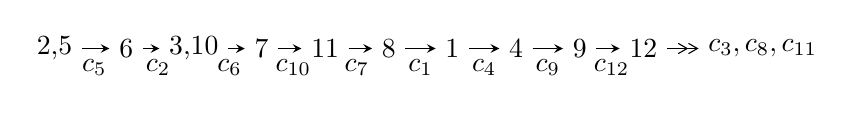
\begin{tikzpicture}[x=23pt, y=7pt]
	% node
	\node (A0) at (-1/8, 0) {2,5};
	\node (A1) at (1, 0) {6};
	\node (A2) at (33/16, 0) {3,10};
	\node (A3) at (25/8, 0) {7};
	\node (A4) at (33/8, 0) {11};
	\node (A5) at (41/8, 0) {8};
	\node (A6) at (49/8, 0) {1};
	\node (A7) at (57/8, 0) {4};
	\node (A8) at (65/8, 0) {9};
	\node (A9) at (73/8, 0) {12};
	\node (C1) at (1/2, -1) {$c_{5}$};
	\node (C2) at (3/2, -1) {$c_{2}$};
	\node (C3) at (21/8, -1) {$c_{6}$};
	\node (C4) at (29/8, -1) {$c_{10}$};
	\node (C5) at (37/8, -1) {$c_{7}$};
	\node (C6) at (45/8, -1) {$c_{1}$};
	\node (C7) at (53/8, -1) {$c_{4}$};
	\node (C8) at (61/8, -1) {$c_{9}$};
	\node (C9) at (69/8, -1) {$c_{12}$};
	\node (A10) at (11, 0) {$c_{3},c_{8},c_{11}$};

	% edge
	\draw[->,>=stealth]	
	(A0) edge (A1) (A1) edge (A2) (A2) edge (A3) (A3) edge (A4) (A4) edge (A5) (A5) edge (A6) (A6) edge (A7) (A7) edge (A8) (A8) edge (A9) ;
	\draw[->>,>={angle 60}]	
	(A9) edge (A10);
\end{tikzpicture} \\ 

\end{tabular} \\

\footnotetext{
The image of knot diagram is generated by the software ``\textbf{Draw programme}" developed by Andrew Bartholomew(\url{http://www.layer8.co.uk/maths/draw/index.htm\#Running-draw}), where we modified some parts for our purpose(\url{https://github.com/CATsTAILs/LinksPainter}).
}\phantom \\ \newline 
\centering \textbf{Ideals for irreducible components\footnotemark of $X_{\text{par}}$} 
 
\begin{align*}
I^u_{1}&=\langle 
4.53998\times10^{26} u^{51}+5.05817\times10^{27} u^{50}+\cdots+2.07754\times10^{25} b-7.39267\times10^{27},\\
\phantom{I^u_{1}}&\phantom{= \langle  }6.84425\times10^{27} u^{51}+7.36349\times10^{28} u^{50}+\cdots+1.66203\times10^{26} a-9.03557\times10^{28},\\
\phantom{I^u_{1}}&\phantom{= \langle  }u^{52}+11 u^{51}+\cdots-105 u-8\rangle \\
I^u_{2}&=\langle 
-2 u^{41} a-45 u^{41}+\cdots+6 a+347,\;825 u^{41} a-163 u^{41}+\cdots-6825 a-727,\;u^{42}-4 u^{41}+\cdots-23 u+3\rangle \\
I^u_{3}&=\langle 
-3 u^{15}+11 u^{14}+\cdots+b+6,\;-4 u^{15}+13 u^{14}+\cdots+a+6,\\
\phantom{I^u_{3}}&\phantom{= \langle  }u^{16}-4 u^{15}+5 u^{14}+4 u^{13}-19 u^{12}+23 u^{11}-11 u^{10}-3 u^9+15 u^8-29 u^7+35 u^6-22 u^5+5 u^4+3 u^2-3 u+1\rangle \\
I^u_{4}&=\langle 
- u^3 a- u^2 a+u^3+a u+2 b+1,\;u^2 a+3 u^3+a^2+a u+2 u^2- a-3 u-2,\;u^4- u^2+1\rangle \\
I^u_{5}&=\langle 
b- a-1,\;a^2+3 a+3,\;u+1\rangle \\
I^u_{6}&=\langle 
b- a+1,\;a^4-6 a^3+15 a^2-18 a+7,\;u+1\rangle \\
\\
\end{align*}
\raggedright * 6 irreducible components of $\dim_{\mathbb{C}}=0$, with total 166 representations.\\
\footnotetext{All coefficients of polynomials are rational numbers. But the coefficients are sometimes approximated in decimal forms when there is not enough margin.}
\newpage
\renewcommand{\arraystretch}{1}
\centering \section*{I. $I^u_{1}= \langle 4.54\times10^{26} u^{51}+5.06\times10^{27} u^{50}+\cdots+2.08\times10^{25} b-7.39\times10^{27},\;6.84\times10^{27} u^{51}+7.36\times10^{28} u^{50}+\cdots+1.66\times10^{26} a-9.04\times10^{28},\;u^{52}+11 u^{51}+\cdots-105 u-8 \rangle$}
\flushleft \textbf{(i) Arc colorings}\\
\begin{tabular}{m{7pt} m{180pt} m{7pt} m{180pt} }
\flushright $a_{2}=$&$\begin{pmatrix}0\\u\end{pmatrix}$ \\
\flushright $a_{5}=$&$\begin{pmatrix}1\\0\end{pmatrix}$ \\
\flushright $a_{6}=$&$\begin{pmatrix}1\\u^2\end{pmatrix}$ \\
\flushright $a_{3}=$&$\begin{pmatrix}- u\\- u^3+u\end{pmatrix}$ \\
\flushright $a_{10}=$&$\begin{pmatrix}-41.1800 u^{51}-443.041 u^{50}+\cdots+6409.16 u+543.645\\-21.8527 u^{51}-243.469 u^{50}+\cdots+4181.40 u+355.837\end{pmatrix}$ \\
\flushright $a_{7}=$&$\begin{pmatrix}-7.78427 u^{51}-87.7140 u^{50}+\cdots+1359.23 u+119.895\\5.98217 u^{51}+53.3671 u^{50}+\cdots+74.8168 u+11.4814\end{pmatrix}$ \\
\flushright $a_{11}=$&$\begin{pmatrix}-19.3273 u^{51}-199.572 u^{50}+\cdots+2227.76 u+187.808\\-21.8527 u^{51}-243.469 u^{50}+\cdots+4181.40 u+355.837\end{pmatrix}$ \\
\flushright $a_{8}=$&$\begin{pmatrix}4.76000 u^{51}+46.4262 u^{50}+\cdots-283.578 u-23.1030\\-33.4051 u^{51}-334.756 u^{50}+\cdots+3096.45 u+251.825\end{pmatrix}$ \\
\flushright $a_{1}=$&$\begin{pmatrix}u^3\\u^5- u^3+u\end{pmatrix}$ \\
\flushright $a_{4}=$&$\begin{pmatrix}-7.06370 u^{51}-73.7381 u^{50}+\cdots+927.555 u+84.2568\\9.30260 u^{51}+91.2779 u^{50}+\cdots-515.128 u-37.6927\end{pmatrix}$ \\
\flushright $a_{9}=$&$\begin{pmatrix}-31.4511 u^{51}-330.139 u^{50}+\cdots+3966.66 u+334.341\\-9.22694 u^{51}-119.633 u^{50}+\cdots+3251.38 u+281.203\end{pmatrix}$ \\
\flushright $a_{12}=$&$\begin{pmatrix}37.4120 u^{51}+372.930 u^{50}+\cdots-3121.91 u-246.831\\28.4339 u^{51}+293.834 u^{50}+\cdots-3277.17 u-270.732\end{pmatrix}$\\&\end{tabular}
\flushleft \textbf{(ii) Obstruction class $= -1$}\\~\\
\flushleft \textbf{(iii) Cusp Shapes $= -\frac{552510409213253669452495646}{4155086772164184949828265} u^{51}-\frac{5261625346514302913687205342}{4155086772164184949828265} u^{50}+\cdots+\frac{21341655761740046577824999282}{4155086772164184949828265} u+\frac{1496242834046200807960011522}{4155086772164184949828265}$}\\~\\
\newpage\renewcommand{\arraystretch}{1}
\flushleft \textbf{(iv) u-Polynomials at the component}\newline \\
\begin{tabular}{m{50pt}|m{274pt}}
Crossings & \hspace{64pt}u-Polynomials at each crossing \\
\hline $$\begin{aligned}c_{1}\end{aligned}$$&$\begin{aligned}
&u^{52}+19 u^{51}+\cdots+2465 u+64
\end{aligned}$\\
\hline $$\begin{aligned}c_{2},c_{5}\end{aligned}$$&$\begin{aligned}
&u^{52}+11 u^{51}+\cdots-105 u-8
\end{aligned}$\\
\hline $$\begin{aligned}c_{3},c_{10}\end{aligned}$$&$\begin{aligned}
&u^{52}+12 u^{50}+\cdots-11 u+1
\end{aligned}$\\
\hline $$\begin{aligned}c_{4},c_{12}\end{aligned}$$&$\begin{aligned}
&u^{52}+4 u^{51}+\cdots-11 u+1
\end{aligned}$\\
\hline $$\begin{aligned}c_{6},c_{9}\end{aligned}$$&$\begin{aligned}
&u^{52}-4 u^{51}+\cdots+u-1
\end{aligned}$\\
\hline $$\begin{aligned}c_{7},c_{8},c_{11}\end{aligned}$$&$\begin{aligned}
&u^{52}-14 u^{51}+\cdots-15 u+2
\end{aligned}$\\
\hline
\end{tabular}\\~\\
\newpage\renewcommand{\arraystretch}{1}
\flushleft \textbf{(v) Riley Polynomials at the component}\newline \\
\begin{tabular}{m{50pt}|m{274pt}}
Crossings & \hspace{64pt}Riley Polynomials at each crossing \\
\hline $$\begin{aligned}c_{1}\end{aligned}$$&$\begin{aligned}
&y^{52}+21 y^{51}+\cdots-3151553 y+4096
\end{aligned}$\\
\hline $$\begin{aligned}c_{2},c_{5}\end{aligned}$$&$\begin{aligned}
&y^{52}-19 y^{51}+\cdots-2465 y+64
\end{aligned}$\\
\hline $$\begin{aligned}c_{3},c_{10}\end{aligned}$$&$\begin{aligned}
&y^{52}+24 y^{51}+\cdots-43 y+1
\end{aligned}$\\
\hline $$\begin{aligned}c_{4},c_{12}\end{aligned}$$&$\begin{aligned}
&y^{52}+12 y^{51}+\cdots-31 y+1
\end{aligned}$\\
\hline $$\begin{aligned}c_{6},c_{9}\end{aligned}$$&$\begin{aligned}
&y^{52}-30 y^{51}+\cdots-61 y+1
\end{aligned}$\\
\hline $$\begin{aligned}c_{7},c_{8},c_{11}\end{aligned}$$&$\begin{aligned}
&y^{52}-58 y^{51}+\cdots-137 y+4
\end{aligned}$\\
\hline
\end{tabular}\\~\\
\newpage\flushleft \textbf{(vi) Complex Volumes and Cusp Shapes}
$$\begin{array}{c|c|c}  
\text{Solutions to }I^u_{1}& \I (\text{vol} + \sqrt{-1}CS) & \text{Cusp shape}\\
 \hline 
\begin{aligned}
u &= -0.303052 + 0.952802 I \\
a &= \phantom{-}0.034989 + 0.198223 I \\
b &= \phantom{-}0.503950 - 0.617099 I\end{aligned}
 & \phantom{-}1.05551 + 4.23466 I & \phantom{-0.000000 } 0. - 13.94078 I \\ \hline\begin{aligned}
u &= -0.303052 - 0.952802 I \\
a &= \phantom{-}0.034989 - 0.198223 I \\
b &= \phantom{-}0.503950 + 0.617099 I\end{aligned}
 & \phantom{-}1.05551 - 4.23466 I & \phantom{-0.000000 -}0. + 13.94078 I \\ \hline\begin{aligned}
u &= \phantom{-}0.866782 + 0.510957 I \\
a &= \phantom{-}1.83194 - 0.77063 I \\
b &= \phantom{-}0.18058 + 1.43268 I\end{aligned}
 & -1.60266 - 2.06605 I & \phantom{-0.000000 } 0 \\ \hline\begin{aligned}
u &= \phantom{-}0.866782 - 0.510957 I \\
a &= \phantom{-}1.83194 + 0.77063 I \\
b &= \phantom{-}0.18058 - 1.43268 I\end{aligned}
 & -1.60266 + 2.06605 I & \phantom{-0.000000 } 0 \\ \hline\begin{aligned}
u &= -0.878833 + 0.450841 I \\
a &= \phantom{-}0.518755 + 1.197230 I \\
b &= \phantom{-}0.639394 + 0.765044 I\end{aligned}
 & -1.82299 + 2.11483 I & \phantom{-0.000000 } 0 \\ \hline\begin{aligned}
u &= -0.878833 - 0.450841 I \\
a &= \phantom{-}0.518755 - 1.197230 I \\
b &= \phantom{-}0.639394 - 0.765044 I\end{aligned}
 & -1.82299 - 2.11483 I & \phantom{-0.000000 } 0 \\ \hline\begin{aligned}
u &= \phantom{-}0.859521 + 0.581846 I \\
a &= -1.92008 + 0.82944 I \\
b &= -0.07577 - 1.77245 I\end{aligned}
 & \phantom{-}3.98340 - 2.30844 I & \phantom{-0.000000 } 0 \\ \hline\begin{aligned}
u &= \phantom{-}0.859521 - 0.581846 I \\
a &= -1.92008 - 0.82944 I \\
b &= -0.07577 + 1.77245 I\end{aligned}
 & \phantom{-}3.98340 + 2.30844 I & \phantom{-0.000000 } 0 \\ \hline\begin{aligned}
u &= \phantom{-}0.866761 + 0.407706 I \\
a &= -1.43190 + 1.02282 I \\
b &= -0.455587 - 0.870700 I\end{aligned}
 & \phantom{-}1.79191 - 1.98663 I & \phantom{-0.000000 -}0. + 5.10991 I \\ \hline\begin{aligned}
u &= \phantom{-}0.866761 - 0.407706 I \\
a &= -1.43190 - 1.02282 I \\
b &= -0.455587 + 0.870700 I\end{aligned}
 & \phantom{-}1.79191 + 1.98663 I & \phantom{-0.000000 } 0. - 5.10991 I\\
 \hline 
 \end{array}$$\newpage$$\begin{array}{c|c|c}  
\text{Solutions to }I^u_{1}& \I (\text{vol} + \sqrt{-1}CS) & \text{Cusp shape}\\
 \hline 
\begin{aligned}
u &= -0.949503 + 0.456951 I \\
a &= -1.23169 - 1.28904 I \\
b &= -1.275250 - 0.565238 I\end{aligned}
 & \phantom{-}2.17857 + 3.11727 I & \phantom{-0.000000 } 0 \\ \hline\begin{aligned}
u &= -0.949503 - 0.456951 I \\
a &= -1.23169 + 1.28904 I \\
b &= -1.275250 + 0.565238 I\end{aligned}
 & \phantom{-}2.17857 - 3.11727 I & \phantom{-0.000000 } 0 \\ \hline\begin{aligned}
u &= \phantom{-}1.059230 + 0.081807 I \\
a &= \phantom{-}1.80017 + 0.56735 I \\
b &= \phantom{-}0.686878 + 0.509668 I\end{aligned}
 & -4.61713 - 2.77958 I & \phantom{-0.000000 } 0 \\ \hline\begin{aligned}
u &= \phantom{-}1.059230 - 0.081807 I \\
a &= \phantom{-}1.80017 - 0.56735 I \\
b &= \phantom{-}0.686878 - 0.509668 I\end{aligned}
 & -4.61713 + 2.77958 I & \phantom{-0.000000 } 0 \\ \hline\begin{aligned}
u &= -0.677772 + 0.818492 I \\
a &= -0.417172 + 0.333279 I \\
b &= -0.602964 - 0.807052 I\end{aligned}
 & \phantom{-}1.60486 - 2.99292 I & \phantom{-0.000000 } 0 \\ \hline\begin{aligned}
u &= -0.677772 - 0.818492 I \\
a &= -0.417172 - 0.333279 I \\
b &= -0.602964 + 0.807052 I\end{aligned}
 & \phantom{-}1.60486 + 2.99292 I & \phantom{-0.000000 } 0 \\ \hline\begin{aligned}
u &= -0.592287 + 0.905759 I \\
a &= \phantom{-}0.073021 - 0.240968 I \\
b &= \phantom{-}0.759625 + 1.129160 I\end{aligned}
 & \phantom{-}2.71314 - 8.81698 I & \phantom{-0.000000 } 0 \\ \hline\begin{aligned}
u &= -0.592287 - 0.905759 I \\
a &= \phantom{-}0.073021 + 0.240968 I \\
b &= \phantom{-}0.759625 - 1.129160 I\end{aligned}
 & \phantom{-}2.71314 + 8.81698 I & \phantom{-0.000000 } 0 \\ \hline\begin{aligned}
u &= \phantom{-}0.754853 + 0.482158 I \\
a &= -1.006070 + 0.984106 I \\
b &= -0.206125 - 0.823600 I\end{aligned}
 & \phantom{-}1.78251 - 2.04552 I & \phantom{-}5.02176 + 4.06371 I \\ \hline\begin{aligned}
u &= \phantom{-}0.754853 - 0.482158 I \\
a &= -1.006070 - 0.984106 I \\
b &= -0.206125 + 0.823600 I\end{aligned}
 & \phantom{-}1.78251 + 2.04552 I & \phantom{-}5.02176 - 4.06371 I\\
 \hline 
 \end{array}$$\newpage$$\begin{array}{c|c|c}  
\text{Solutions to }I^u_{1}& \I (\text{vol} + \sqrt{-1}CS) & \text{Cusp shape}\\
 \hline 
\begin{aligned}
u &= -0.809152 + 0.343854 I \\
a &= \phantom{-}0.19899 - 1.72190 I \\
b &= -0.16082 - 1.41998 I\end{aligned}
 & \phantom{-}2.68462 + 1.40366 I & \phantom{-}1.58938 - 4.99897 I \\ \hline\begin{aligned}
u &= -0.809152 - 0.343854 I \\
a &= \phantom{-}0.19899 + 1.72190 I \\
b &= -0.16082 + 1.41998 I\end{aligned}
 & \phantom{-}2.68462 - 1.40366 I & \phantom{-}1.58938 + 4.99897 I \\ \hline\begin{aligned}
u &= -0.571688 + 0.974680 I \\
a &= \phantom{-}0.079015 + 0.294171 I \\
b &= -0.78314 - 1.37043 I\end{aligned}
 & \phantom{-}10.3015 - 12.7497 I & \phantom{-0.000000 } 0 \\ \hline\begin{aligned}
u &= -0.571688 - 0.974680 I \\
a &= \phantom{-}0.079015 - 0.294171 I \\
b &= -0.78314 + 1.37043 I\end{aligned}
 & \phantom{-}10.3015 + 12.7497 I & \phantom{-0.000000 } 0 \\ \hline\begin{aligned}
u &= -1.097450 + 0.438565 I \\
a &= -0.647329 - 0.449697 I \\
b &= -0.761433 - 0.057762 I\end{aligned}
 & -2.17033 + 0.83260 I & \phantom{-0.000000 } 0 \\ \hline\begin{aligned}
u &= -1.097450 - 0.438565 I \\
a &= -0.647329 + 0.449697 I \\
b &= -0.761433 + 0.057762 I\end{aligned}
 & -2.17033 - 0.83260 I & \phantom{-0.000000 } 0 \\ \hline\begin{aligned}
u &= -0.808774\phantom{ +0.000000I} \\
a &= \phantom{-}1.40558\phantom{ +0.000000I} \\
b &= \phantom{-}1.17657\phantom{ +0.000000I}\end{aligned}
 & \phantom{-}3.21409\phantom{ +0.000000I} & \phantom{-}2.59480\phantom{ +0.000000I} \\ \hline\begin{aligned}
u &= -0.983133 + 0.709385 I \\
a &= \phantom{-}0.424839 + 0.547549 I \\
b &= \phantom{-}0.291156 - 0.095304 I\end{aligned}
 & -1.12819 + 2.86961 I & \phantom{-0.000000 } 0 \\ \hline\begin{aligned}
u &= -0.983133 - 0.709385 I \\
a &= \phantom{-}0.424839 - 0.547549 I \\
b &= \phantom{-}0.291156 + 0.095304 I\end{aligned}
 & -1.12819 - 2.86961 I & \phantom{-0.000000 } 0 \\ \hline\begin{aligned}
u &= \phantom{-}1.207840 + 0.122118 I \\
a &= -1.48373 - 0.59924 I \\
b &= -0.901527 - 0.819910 I\end{aligned}
 & -4.39988 - 7.39386 I & \phantom{-0.000000 } 0\\
 \hline 
 \end{array}$$\newpage$$\begin{array}{c|c|c}  
\text{Solutions to }I^u_{1}& \I (\text{vol} + \sqrt{-1}CS) & \text{Cusp shape}\\
 \hline 
\begin{aligned}
u &= \phantom{-}1.207840 - 0.122118 I \\
a &= -1.48373 + 0.59924 I \\
b &= -0.901527 + 0.819910 I\end{aligned}
 & -4.39988 + 7.39386 I & \phantom{-0.000000 } 0 \\ \hline\begin{aligned}
u &= -0.878018 + 0.876003 I \\
a &= -0.078786 - 0.959376 I \\
b &= -0.020706 + 0.697334 I\end{aligned}
 & \phantom{-}8.76056 + 3.51365 I & \phantom{-0.000000 } 0 \\ \hline\begin{aligned}
u &= -0.878018 - 0.876003 I \\
a &= -0.078786 + 0.959376 I \\
b &= -0.020706 - 0.697334 I\end{aligned}
 & \phantom{-}8.76056 - 3.51365 I & \phantom{-0.000000 } 0 \\ \hline\begin{aligned}
u &= -1.027700 + 0.716646 I \\
a &= \phantom{-}1.67678 + 0.76544 I \\
b &= \phantom{-}0.700230 - 0.834328 I\end{aligned}
 & \phantom{-}0.53141 + 8.76844 I & \phantom{-0.000000 } 0 \\ \hline\begin{aligned}
u &= -1.027700 - 0.716646 I \\
a &= \phantom{-}1.67678 - 0.76544 I \\
b &= \phantom{-}0.700230 + 0.834328 I\end{aligned}
 & \phantom{-}0.53141 - 8.76844 I & \phantom{-0.000000 } 0 \\ \hline\begin{aligned}
u &= \phantom{-}0.915507 + 0.868903 I \\
a &= \phantom{-}0.654011 - 0.348314 I \\
b &= -0.000634 + 1.130420 I\end{aligned}
 & \phantom{-}10.44970 - 3.21474 I & \phantom{-0.000000 } 0 \\ \hline\begin{aligned}
u &= \phantom{-}0.915507 - 0.868903 I \\
a &= \phantom{-}0.654011 + 0.348314 I \\
b &= -0.000634 - 1.130420 I\end{aligned}
 & \phantom{-}10.44970 + 3.21474 I & \phantom{-0.000000 } 0 \\ \hline\begin{aligned}
u &= -0.969489 + 0.820816 I \\
a &= -0.978341 - 0.759518 I \\
b &= -0.058160 + 0.678489 I\end{aligned}
 & \phantom{-}8.44609 + 2.83761 I & \phantom{-0.000000 } 0 \\ \hline\begin{aligned}
u &= -0.969489 - 0.820816 I \\
a &= -0.978341 + 0.759518 I \\
b &= -0.058160 - 0.678489 I\end{aligned}
 & \phantom{-}8.44609 - 2.83761 I & \phantom{-0.000000 } 0 \\ \hline\begin{aligned}
u &= -0.305651 + 1.237930 I \\
a &= \phantom{-}0.088791 - 0.250502 I \\
b &= -0.643580 + 0.726750 I\end{aligned}
 & \phantom{-}8.73516 + 6.32971 I & \phantom{-0.000000 } 0\\
 \hline 
 \end{array}$$\newpage$$\begin{array}{c|c|c}  
\text{Solutions to }I^u_{1}& \I (\text{vol} + \sqrt{-1}CS) & \text{Cusp shape}\\
 \hline 
\begin{aligned}
u &= -0.305651 - 1.237930 I \\
a &= \phantom{-}0.088791 + 0.250502 I \\
b &= -0.643580 - 0.726750 I\end{aligned}
 & \phantom{-}8.73516 - 6.32971 I & \phantom{-0.000000 } 0 \\ \hline\begin{aligned}
u &= -1.087350 + 0.717339 I \\
a &= -1.76484 - 0.61554 I \\
b &= -0.85686 + 1.19595 I\end{aligned}
 & \phantom{-}1.1878 + 14.8065 I & \phantom{-0.000000 } 0 \\ \hline\begin{aligned}
u &= -1.087350 - 0.717339 I \\
a &= -1.76484 + 0.61554 I \\
b &= -0.85686 - 1.19595 I\end{aligned}
 & \phantom{-}1.1878 - 14.8065 I & \phantom{-0.000000 } 0 \\ \hline\begin{aligned}
u &= \phantom{-}0.692693\phantom{ +0.000000I} \\
a &= -2.67905\phantom{ +0.000000I} \\
b &= \phantom{-}0.160423\phantom{ +0.000000I}\end{aligned}
 & \phantom{-}2.79063\phantom{ +0.000000I} & \phantom{-}9.38280\phantom{ +0.000000I} \\ \hline\begin{aligned}
u &= \phantom{-}1.311730 + 0.155198 I \\
a &= \phantom{-}1.29329 + 0.62840 I \\
b &= \phantom{-}0.98298 + 1.07363 I\end{aligned}
 & \phantom{-}2.56871 - 10.65480 I & \phantom{-0.000000 } 0 \\ \hline\begin{aligned}
u &= \phantom{-}1.311730 - 0.155198 I \\
a &= \phantom{-}1.29329 - 0.62840 I \\
b &= \phantom{-}0.98298 - 1.07363 I\end{aligned}
 & \phantom{-}2.56871 + 10.65480 I & \phantom{-0.000000 } 0 \\ \hline\begin{aligned}
u &= -1.121430 + 0.731849 I \\
a &= \phantom{-}1.80711 + 0.50804 I \\
b &= \phantom{-}0.85609 - 1.46709 I\end{aligned}
 & \phantom{-}8.5842 + 18.9717 I & \phantom{-0.000000 } 0 \\ \hline\begin{aligned}
u &= -1.121430 - 0.731849 I \\
a &= \phantom{-}1.80711 - 0.50804 I \\
b &= \phantom{-}0.85609 + 1.46709 I\end{aligned}
 & \phantom{-}8.5842 - 18.9717 I & \phantom{-0.000000 } 0 \\ \hline\begin{aligned}
u &= -1.41178\phantom{ +0.000000I} \\
a &= \phantom{-}0.588810\phantom{ +0.000000I} \\
b &= \phantom{-}0.957114\phantom{ +0.000000I}\end{aligned}
 & \phantom{-}3.53219\phantom{ +0.000000I} & \phantom{-0.000000 } 0 \\ \hline\begin{aligned}
u &= -0.231217 + 0.451747 I \\
a &= -0.804630 - 0.251513 I \\
b &= -0.392803 + 0.547987 I\end{aligned}
 & -0.630419 + 1.163880 I & -3.53445 - 4.93440 I\\
 \hline 
 \end{array}$$\newpage$$\begin{array}{c|c|c}  
\text{Solutions to }I^u_{1}& \I (\text{vol} + \sqrt{-1}CS) & \text{Cusp shape}\\
 \hline 
\begin{aligned}
u &= -0.231217 - 0.451747 I \\
a &= -0.804630 + 0.251513 I \\
b &= -0.392803 - 0.547987 I\end{aligned}
 & -0.630419 - 1.163880 I & -3.53445 + 4.93440 I \\ \hline\begin{aligned}
u &= -0.189131\phantom{ +0.000000I} \\
a &= \phantom{-}4.12539\phantom{ +0.000000I} \\
b &= \phantom{-}0.894842\phantom{ +0.000000I}\end{aligned}
 & \phantom{-}3.37184\phantom{ +0.000000I} & \phantom{-}1.02460\phantom{ +0.000000I}\\
 \hline 
 \end{array}$$\newpage\newpage\renewcommand{\arraystretch}{1}
\centering \section*{II. $I^u_{2}= \langle -2 u^{41} a-45 u^{41}+\cdots+6 a+347,\;825 u^{41} a-163 u^{41}+\cdots-6825 a-727,\;u^{42}-4 u^{41}+\cdots-23 u+3 \rangle$}
\flushleft \textbf{(i) Arc colorings}\\
\begin{tabular}{m{7pt} m{180pt} m{7pt} m{180pt} }
\flushright $a_{2}=$&$\begin{pmatrix}0\\u\end{pmatrix}$ \\
\flushright $a_{5}=$&$\begin{pmatrix}1\\0\end{pmatrix}$ \\
\flushright $a_{6}=$&$\begin{pmatrix}1\\u^2\end{pmatrix}$ \\
\flushright $a_{3}=$&$\begin{pmatrix}- u\\- u^3+u\end{pmatrix}$ \\
\flushright $a_{10}=$&$\begin{pmatrix}a\\\frac{1}{2} u^{41} a+\frac{45}{4} u^{41}+\cdots-\frac{3}{2} a-\frac{347}{4}\end{pmatrix}$ \\
\flushright $a_{7}=$&$\begin{pmatrix}-6.25000 a u^{41}-1.83333 u^{41}+\cdots+15.7500 a+19.6667\\\frac{23}{4} u^{41} a-\frac{87}{4} u^{40} a+\cdots-\frac{147}{4} a-1\end{pmatrix}$ \\
\flushright $a_{11}=$&$\begin{pmatrix}-0.500000 a u^{41}-11.2500 u^{41}+\cdots+2.50000 a+86.7500\\\frac{1}{2} u^{41} a+\frac{45}{4} u^{41}+\cdots-\frac{3}{2} a-\frac{347}{4}\end{pmatrix}$ \\
\flushright $a_{8}=$&$\begin{pmatrix}-9.75000 a u^{41}-5.58333 u^{41}+\cdots+34.2500 a+21.4167\\-\frac{9}{2} u^{41} a+\frac{15}{4} u^{41}+\cdots+15 a-\frac{11}{4}\end{pmatrix}$ \\
\flushright $a_{1}=$&$\begin{pmatrix}u^3\\u^5- u^3+u\end{pmatrix}$ \\
\flushright $a_{4}=$&$\begin{pmatrix}13 u^{41} a-\frac{59}{12} u^{41}+\cdots-\frac{181}{2} a+\frac{43}{12}\\-\frac{9}{4} u^{41} a+\frac{1}{4} u^{41}+\cdots+\frac{69}{4} a-\frac{7}{4}\end{pmatrix}$ \\
\flushright $a_{9}=$&$\begin{pmatrix}\frac{1}{2} u^{41} a+\frac{9}{4} u^{41}+\cdots-\frac{1}{2} a+\frac{9}{4}\\-\frac{1}{2} u^{41} a+\frac{19}{2} u^{41}+\cdots+\frac{3}{2} a-83\end{pmatrix}$ \\
\flushright $a_{12}=$&$\begin{pmatrix}-1.25000 a u^{41}-1.58333 u^{41}+\cdots+14.2500 a+17.9167\\\frac{23}{2} u^{41} a+\frac{1}{2} u^{41}+\cdots-36 a-\frac{5}{2}\end{pmatrix}$\\&\end{tabular}
\flushleft \textbf{(ii) Obstruction class $= -1$}\\~\\
\flushleft \textbf{(iii) Cusp Shapes $= -\frac{201}{4} u^{41}+\frac{677}{4} u^{40}+\cdots-\frac{2695}{2} u+\frac{853}{4}$}\\~\\
\newpage\renewcommand{\arraystretch}{1}
\flushleft \textbf{(iv) u-Polynomials at the component}\newline \\
\begin{tabular}{m{50pt}|m{274pt}}
Crossings & \hspace{64pt}u-Polynomials at each crossing \\
\hline $$\begin{aligned}c_{1}\end{aligned}$$&$\begin{aligned}
&(u^{42}+18 u^{41}+\cdots+139 u+9)^{2}
\end{aligned}$\\
\hline $$\begin{aligned}c_{2},c_{5}\end{aligned}$$&$\begin{aligned}
&(u^{42}-4 u^{41}+\cdots-23 u+3)^{2}
\end{aligned}$\\
\hline $$\begin{aligned}c_{3},c_{10}\end{aligned}$$&$\begin{aligned}
&u^{84}-2 u^{83}+\cdots+277053 u-23701
\end{aligned}$\\
\hline $$\begin{aligned}c_{4},c_{12}\end{aligned}$$&$\begin{aligned}
&u^{84}+10 u^{83}+\cdots-117 u+513
\end{aligned}$\\
\hline $$\begin{aligned}c_{6},c_{9}\end{aligned}$$&$\begin{aligned}
&u^{84}- u^{83}+\cdots+8 u-1
\end{aligned}$\\
\hline $$\begin{aligned}c_{7},c_{8},c_{11}\end{aligned}$$&$\begin{aligned}
&(u^{42}+5 u^{41}+\cdots-8 u-2)^{2}
\end{aligned}$\\
\hline
\end{tabular}\\~\\
\newpage\renewcommand{\arraystretch}{1}
\flushleft \textbf{(v) Riley Polynomials at the component}\newline \\
\begin{tabular}{m{50pt}|m{274pt}}
Crossings & \hspace{64pt}Riley Polynomials at each crossing \\
\hline $$\begin{aligned}c_{1}\end{aligned}$$&$\begin{aligned}
&(y^{42}+18 y^{41}+\cdots+317 y+81)^{2}
\end{aligned}$\\
\hline $$\begin{aligned}c_{2},c_{5}\end{aligned}$$&$\begin{aligned}
&(y^{42}-18 y^{41}+\cdots-139 y+9)^{2}
\end{aligned}$\\
\hline $$\begin{aligned}c_{3},c_{10}\end{aligned}$$&$\begin{aligned}
&y^{84}+30 y^{83}+\cdots-54716197799 y+561737401
\end{aligned}$\\
\hline $$\begin{aligned}c_{4},c_{12}\end{aligned}$$&$\begin{aligned}
&y^{84}-34 y^{83}+\cdots-6200469 y+263169
\end{aligned}$\\
\hline $$\begin{aligned}c_{6},c_{9}\end{aligned}$$&$\begin{aligned}
&y^{84}+17 y^{83}+\cdots-72 y+1
\end{aligned}$\\
\hline $$\begin{aligned}c_{7},c_{8},c_{11}\end{aligned}$$&$\begin{aligned}
&(y^{42}-45 y^{41}+\cdots-96 y+4)^{2}
\end{aligned}$\\
\hline
\end{tabular}\\~\\
\newpage\flushleft \textbf{(vi) Complex Volumes and Cusp Shapes}
$$\begin{array}{c|c|c}  
\text{Solutions to }I^u_{2}& \I (\text{vol} + \sqrt{-1}CS) & \text{Cusp shape}\\
 \hline 
\begin{aligned}
u &= \phantom{-}0.510010 + 0.891471 I \\
a &= -0.217501 + 0.082995 I \\
b &= \phantom{-}0.709398 - 1.077620 I\end{aligned}
 & \phantom{-}3.96533 + 2.20033 I & \phantom{-}7.78344 - 3.54101 I \\ \hline\begin{aligned}
u &= \phantom{-}0.510010 + 0.891471 I \\
a &= -0.204654 - 0.010293 I \\
b &= -0.194625 + 0.780336 I\end{aligned}
 & \phantom{-}3.96533 + 2.20033 I & \phantom{-}7.78344 - 3.54101 I \\ \hline\begin{aligned}
u &= \phantom{-}0.510010 - 0.891471 I \\
a &= -0.217501 - 0.082995 I \\
b &= \phantom{-}0.709398 + 1.077620 I\end{aligned}
 & \phantom{-}3.96533 - 2.20033 I & \phantom{-}7.78344 + 3.54101 I \\ \hline\begin{aligned}
u &= \phantom{-}0.510010 - 0.891471 I \\
a &= -0.204654 + 0.010293 I \\
b &= -0.194625 - 0.780336 I\end{aligned}
 & \phantom{-}3.96533 - 2.20033 I & \phantom{-}7.78344 + 3.54101 I \\ \hline\begin{aligned}
u &= \phantom{-}0.730561 + 0.637744 I \\
a &= -0.161192 + 1.028670 I \\
b &= \phantom{-}0.163687 - 0.913124 I\end{aligned}
 & \phantom{-}1.88224 - 1.77676 I & \phantom{-}3.40533 + 1.54020 I \\ \hline\begin{aligned}
u &= \phantom{-}0.730561 + 0.637744 I \\
a &= -1.091270 + 0.713205 I \\
b &= -0.624504 - 0.895096 I\end{aligned}
 & \phantom{-}1.88224 - 1.77676 I & \phantom{-}3.40533 + 1.54020 I \\ \hline\begin{aligned}
u &= \phantom{-}0.730561 - 0.637744 I \\
a &= -0.161192 - 1.028670 I \\
b &= \phantom{-}0.163687 + 0.913124 I\end{aligned}
 & \phantom{-}1.88224 + 1.77676 I & \phantom{-}3.40533 - 1.54020 I \\ \hline\begin{aligned}
u &= \phantom{-}0.730561 - 0.637744 I \\
a &= -1.091270 - 0.713205 I \\
b &= -0.624504 + 0.895096 I\end{aligned}
 & \phantom{-}1.88224 + 1.77676 I & \phantom{-}3.40533 - 1.54020 I \\ \hline\begin{aligned}
u &= -0.779828 + 0.674893 I \\
a &= -0.435770 - 0.013571 I \\
b &= \phantom{-}0.72936 + 1.57734 I\end{aligned}
 & \phantom{-}10.25860 - 4.34016 I & \phantom{-}5.15506 + 1.20379 I \\ \hline\begin{aligned}
u &= -0.779828 + 0.674893 I \\
a &= \phantom{-}2.07249 + 0.66236 I \\
b &= -0.136878 - 0.796276 I\end{aligned}
 & \phantom{-}10.25860 - 4.34016 I & \phantom{-}5.15506 + 1.20379 I\\
 \hline 
 \end{array}$$\newpage$$\begin{array}{c|c|c}  
\text{Solutions to }I^u_{2}& \I (\text{vol} + \sqrt{-1}CS) & \text{Cusp shape}\\
 \hline 
\begin{aligned}
u &= -0.779828 - 0.674893 I \\
a &= -0.435770 + 0.013571 I \\
b &= \phantom{-}0.72936 - 1.57734 I\end{aligned}
 & \phantom{-}10.25860 + 4.34016 I & \phantom{-}5.15506 - 1.20379 I \\ \hline\begin{aligned}
u &= -0.779828 - 0.674893 I \\
a &= \phantom{-}2.07249 - 0.66236 I \\
b &= -0.136878 + 0.796276 I\end{aligned}
 & \phantom{-}10.25860 + 4.34016 I & \phantom{-}5.15506 - 1.20379 I \\ \hline\begin{aligned}
u &= -0.822928 + 0.631892 I \\
a &= -0.176436 - 0.110160 I \\
b &= -0.733366 - 1.134380 I\end{aligned}
 & \phantom{-}3.00889 - 0.33164 I & \phantom{-}4.36259 + 0. I\phantom{ +0.000000I} \\ \hline\begin{aligned}
u &= -0.822928 + 0.631892 I \\
a &= -2.08391 - 0.64936 I \\
b &= -0.347636 + 0.639214 I\end{aligned}
 & \phantom{-}3.00889 - 0.33164 I & \phantom{-}4.36259 + 0. I\phantom{ +0.000000I} \\ \hline\begin{aligned}
u &= -0.822928 - 0.631892 I \\
a &= -0.176436 + 0.110160 I \\
b &= -0.733366 + 1.134380 I\end{aligned}
 & \phantom{-}3.00889 + 0.33164 I & \phantom{-}4.36259 + 0. I\phantom{ +0.000000I} \\ \hline\begin{aligned}
u &= -0.822928 - 0.631892 I \\
a &= -2.08391 + 0.64936 I \\
b &= -0.347636 - 0.639214 I\end{aligned}
 & \phantom{-}3.00889 + 0.33164 I & \phantom{-}4.36259 + 0. I\phantom{ +0.000000I} \\ \hline\begin{aligned}
u &= -0.875027 + 0.294558 I \\
a &= -1.50259 - 1.83848 I \\
b &= -0.183063 - 0.439638 I\end{aligned}
 & -0.96070 + 1.25401 I & -8.94945 + 0.67445 I \\ \hline\begin{aligned}
u &= -0.875027 + 0.294558 I \\
a &= \phantom{-}2.34203 - 0.82616 I \\
b &= \phantom{-}0.35785 - 1.95258 I\end{aligned}
 & -0.96070 + 1.25401 I & -8.94945 + 0.67445 I \\ \hline\begin{aligned}
u &= -0.875027 - 0.294558 I \\
a &= -1.50259 + 1.83848 I \\
b &= -0.183063 + 0.439638 I\end{aligned}
 & -0.96070 - 1.25401 I & -8.94945 - 0.67445 I \\ \hline\begin{aligned}
u &= -0.875027 - 0.294558 I \\
a &= \phantom{-}2.34203 + 0.82616 I \\
b &= \phantom{-}0.35785 + 1.95258 I\end{aligned}
 & -0.96070 - 1.25401 I & -8.94945 - 0.67445 I\\
 \hline 
 \end{array}$$\newpage$$\begin{array}{c|c|c}  
\text{Solutions to }I^u_{2}& \I (\text{vol} + \sqrt{-1}CS) & \text{Cusp shape}\\
 \hline 
\begin{aligned}
u &= -0.876145 + 0.628792 I \\
a &= \phantom{-}0.539905 - 0.602343 I \\
b &= \phantom{-}0.234384 + 0.870708 I\end{aligned}
 & \phantom{-}2.84261 + 5.26736 I & \phantom{-}3.35403 - 7.60586 I \\ \hline\begin{aligned}
u &= -0.876145 + 0.628792 I \\
a &= \phantom{-}2.13558 + 0.80967 I \\
b &= \phantom{-}0.930602 - 1.036450 I\end{aligned}
 & \phantom{-}2.84261 + 5.26736 I & \phantom{-}3.35403 - 7.60586 I \\ \hline\begin{aligned}
u &= -0.876145 - 0.628792 I \\
a &= \phantom{-}0.539905 + 0.602343 I \\
b &= \phantom{-}0.234384 - 0.870708 I\end{aligned}
 & \phantom{-}2.84261 - 5.26736 I & \phantom{-}3.35403 + 7.60586 I \\ \hline\begin{aligned}
u &= -0.876145 - 0.628792 I \\
a &= \phantom{-}2.13558 - 0.80967 I \\
b &= \phantom{-}0.930602 + 1.036450 I\end{aligned}
 & \phantom{-}2.84261 - 5.26736 I & \phantom{-}3.35403 + 7.60586 I \\ \hline\begin{aligned}
u &= \phantom{-}0.527466 + 0.964532 I \\
a &= \phantom{-}0.432004 - 0.205116 I \\
b &= -0.89197 + 1.43000 I\end{aligned}
 & \phantom{-}10.61430 + 2.69864 I & \phantom{-}6.67505 - 1.90999 I \\ \hline\begin{aligned}
u &= \phantom{-}0.527466 + 0.964532 I \\
a &= \phantom{-}0.359003 + 0.138407 I \\
b &= -0.227656 - 0.861311 I\end{aligned}
 & \phantom{-}10.61430 + 2.69864 I & \phantom{-}6.67505 - 1.90999 I \\ \hline\begin{aligned}
u &= \phantom{-}0.527466 - 0.964532 I \\
a &= \phantom{-}0.432004 + 0.205116 I \\
b &= -0.89197 - 1.43000 I\end{aligned}
 & \phantom{-}10.61430 - 2.69864 I & \phantom{-}6.67505 + 1.90999 I \\ \hline\begin{aligned}
u &= \phantom{-}0.527466 - 0.964532 I \\
a &= \phantom{-}0.359003 - 0.138407 I \\
b &= -0.227656 + 0.861311 I\end{aligned}
 & \phantom{-}10.61430 - 2.69864 I & \phantom{-}6.67505 + 1.90999 I \\ \hline\begin{aligned}
u &= -1.093320 + 0.179580 I \\
a &= \phantom{-}0.89041 + 1.21145 I \\
b &= \phantom{-}0.453625 + 0.650671 I\end{aligned}
 & -3.70743 - 0.52130 I & -13.5326 + 9.1617 I \\ \hline\begin{aligned}
u &= -1.093320 + 0.179580 I \\
a &= -1.80070 + 0.29530 I \\
b &= -1.09872 + 1.14420 I\end{aligned}
 & -3.70743 - 0.52130 I & -13.5326 + 9.1617 I\\
 \hline 
 \end{array}$$\newpage$$\begin{array}{c|c|c}  
\text{Solutions to }I^u_{2}& \I (\text{vol} + \sqrt{-1}CS) & \text{Cusp shape}\\
 \hline 
\begin{aligned}
u &= -1.093320 - 0.179580 I \\
a &= \phantom{-}0.89041 - 1.21145 I \\
b &= \phantom{-}0.453625 - 0.650671 I\end{aligned}
 & -3.70743 + 0.52130 I & -13.5326 - 9.1617 I \\ \hline\begin{aligned}
u &= -1.093320 - 0.179580 I \\
a &= -1.80070 - 0.29530 I \\
b &= -1.09872 - 1.14420 I\end{aligned}
 & -3.70743 + 0.52130 I & -13.5326 - 9.1617 I \\ \hline\begin{aligned}
u &= -0.916400 + 0.651883 I \\
a &= -0.207802 + 0.995231 I \\
b &= \phantom{-}0.124308 - 1.016930 I\end{aligned}
 & \phantom{-}9.83608 + 9.47995 I & \phantom{-}3.75244 - 7.98910 I \\ \hline\begin{aligned}
u &= -0.916400 + 0.651883 I \\
a &= -2.29406 - 0.72813 I \\
b &= -0.90398 + 1.59431 I\end{aligned}
 & \phantom{-}9.83608 + 9.47995 I & \phantom{-}3.75244 - 7.98910 I \\ \hline\begin{aligned}
u &= -0.916400 - 0.651883 I \\
a &= -0.207802 - 0.995231 I \\
b &= \phantom{-}0.124308 + 1.016930 I\end{aligned}
 & \phantom{-}9.83608 - 9.47995 I & \phantom{-}3.75244 + 7.98910 I \\ \hline\begin{aligned}
u &= -0.916400 - 0.651883 I \\
a &= -2.29406 + 0.72813 I \\
b &= -0.90398 - 1.59431 I\end{aligned}
 & \phantom{-}9.83608 - 9.47995 I & \phantom{-}3.75244 + 7.98910 I \\ \hline\begin{aligned}
u &= \phantom{-}0.938483 + 0.622081 I \\
a &= -0.290651 - 0.867054 I \\
b &= \phantom{-}0.78135 - 1.19741 I\end{aligned}
 & \phantom{-}1.25328 - 3.16772 I & \phantom{-}1.51749 + 5.49111 I \\ \hline\begin{aligned}
u &= \phantom{-}0.938483 + 0.622081 I \\
a &= -1.82859 + 0.92274 I \\
b &= -0.327871 - 0.874472 I\end{aligned}
 & \phantom{-}1.25328 - 3.16772 I & \phantom{-}1.51749 + 5.49111 I \\ \hline\begin{aligned}
u &= \phantom{-}0.938483 - 0.622081 I \\
a &= -0.290651 + 0.867054 I \\
b &= \phantom{-}0.78135 + 1.19741 I\end{aligned}
 & \phantom{-}1.25328 + 3.16772 I & \phantom{-}1.51749 - 5.49111 I \\ \hline\begin{aligned}
u &= \phantom{-}0.938483 - 0.622081 I \\
a &= -1.82859 - 0.92274 I \\
b &= -0.327871 + 0.874472 I\end{aligned}
 & \phantom{-}1.25328 + 3.16772 I & \phantom{-}1.51749 - 5.49111 I\\
 \hline 
 \end{array}$$\newpage$$\begin{array}{c|c|c}  
\text{Solutions to }I^u_{2}& \I (\text{vol} + \sqrt{-1}CS) & \text{Cusp shape}\\
 \hline 
\begin{aligned}
u &= \phantom{-}0.853008 + 0.796431 I \\
a &= \phantom{-}1.159190 - 0.401879 I \\
b &= -0.155456 + 0.938638 I\end{aligned}
 & \phantom{-}10.22430 - 2.96196 I & \phantom{-}5.75050 + 2.92195 I \\ \hline\begin{aligned}
u &= \phantom{-}0.853008 + 0.796431 I \\
a &= \phantom{-}0.187162 - 0.377050 I \\
b &= \phantom{-}0.104765 + 1.073070 I\end{aligned}
 & \phantom{-}10.22430 - 2.96196 I & \phantom{-}5.75050 + 2.92195 I \\ \hline\begin{aligned}
u &= \phantom{-}0.853008 - 0.796431 I \\
a &= \phantom{-}1.159190 + 0.401879 I \\
b &= -0.155456 - 0.938638 I\end{aligned}
 & \phantom{-}10.22430 + 2.96196 I & \phantom{-}5.75050 - 2.92195 I \\ \hline\begin{aligned}
u &= \phantom{-}0.853008 - 0.796431 I \\
a &= \phantom{-}0.187162 + 0.377050 I \\
b &= \phantom{-}0.104765 - 1.073070 I\end{aligned}
 & \phantom{-}10.22430 + 2.96196 I & \phantom{-}5.75050 - 2.92195 I \\ \hline\begin{aligned}
u &= \phantom{-}1.028580 + 0.594924 I \\
a &= -0.674443 + 1.145360 I \\
b &= -1.47342 + 0.43019 I\end{aligned}
 & -1.01198 - 7.11892 I & -6.76502 + 8.90706 I \\ \hline\begin{aligned}
u &= \phantom{-}1.028580 + 0.594924 I \\
a &= \phantom{-}2.04370 - 0.39791 I \\
b &= \phantom{-}0.626826 + 0.982813 I\end{aligned}
 & -1.01198 - 7.11892 I & -6.76502 + 8.90706 I \\ \hline\begin{aligned}
u &= \phantom{-}1.028580 - 0.594924 I \\
a &= -0.674443 - 1.145360 I \\
b &= -1.47342 - 0.43019 I\end{aligned}
 & -1.01198 + 7.11892 I & -6.76502 - 8.90706 I \\ \hline\begin{aligned}
u &= \phantom{-}1.028580 - 0.594924 I \\
a &= \phantom{-}2.04370 + 0.39791 I \\
b &= \phantom{-}0.626826 - 0.982813 I\end{aligned}
 & -1.01198 + 7.11892 I & -6.76502 - 8.90706 I \\ \hline\begin{aligned}
u &= \phantom{-}0.266931 + 0.728758 I \\
a &= \phantom{-}0.760979 + 0.917167 I \\
b &= -1.413160 + 0.001121 I\end{aligned}
 & \phantom{-}6.40895 + 5.19119 I & \phantom{-}1.23750 - 4.36469 I \\ \hline\begin{aligned}
u &= \phantom{-}0.266931 + 0.728758 I \\
a &= \phantom{-}0.221346 + 0.006852 I \\
b &= \phantom{-}0.580068 - 1.153180 I\end{aligned}
 & \phantom{-}6.40895 + 5.19119 I & \phantom{-}1.23750 - 4.36469 I\\
 \hline 
 \end{array}$$\newpage$$\begin{array}{c|c|c}  
\text{Solutions to }I^u_{2}& \I (\text{vol} + \sqrt{-1}CS) & \text{Cusp shape}\\
 \hline 
\begin{aligned}
u &= \phantom{-}0.266931 - 0.728758 I \\
a &= \phantom{-}0.760979 - 0.917167 I \\
b &= -1.413160 - 0.001121 I\end{aligned}
 & \phantom{-}6.40895 - 5.19119 I & \phantom{-}1.23750 + 4.36469 I \\ \hline\begin{aligned}
u &= \phantom{-}0.266931 - 0.728758 I \\
a &= \phantom{-}0.221346 - 0.006852 I \\
b &= \phantom{-}0.580068 + 1.153180 I\end{aligned}
 & \phantom{-}6.40895 - 5.19119 I & \phantom{-}1.23750 + 4.36469 I \\ \hline\begin{aligned}
u &= \phantom{-}1.101200 + 0.576052 I \\
a &= \phantom{-}1.30305 - 1.16985 I \\
b &= \phantom{-}1.96596 + 0.22334 I\end{aligned}
 & \phantom{-}4.13777 - 10.06040 I & \phantom{-0.000000 } 0 \\ \hline\begin{aligned}
u &= \phantom{-}1.101200 + 0.576052 I \\
a &= -2.01391 + 0.02178 I \\
b &= -0.769329 - 1.160160 I\end{aligned}
 & \phantom{-}4.13777 - 10.06040 I & \phantom{-0.000000 } 0 \\ \hline\begin{aligned}
u &= \phantom{-}1.101200 - 0.576052 I \\
a &= \phantom{-}1.30305 + 1.16985 I \\
b &= \phantom{-}1.96596 - 0.22334 I\end{aligned}
 & \phantom{-}4.13777 + 10.06040 I & \phantom{-0.000000 } 0 \\ \hline\begin{aligned}
u &= \phantom{-}1.101200 - 0.576052 I \\
a &= -2.01391 - 0.02178 I \\
b &= -0.769329 + 1.160160 I\end{aligned}
 & \phantom{-}4.13777 + 10.06040 I & \phantom{-0.000000 } 0 \\ \hline\begin{aligned}
u &= -1.226880 + 0.231515 I \\
a &= -0.399605 - 1.256660 I \\
b &= -0.499288 - 0.861891 I\end{aligned}
 & \phantom{-}1.74664 - 2.01379 I & \phantom{-0.000000 } 0 \\ \hline\begin{aligned}
u &= -1.226880 + 0.231515 I \\
a &= \phantom{-}1.77450 + 0.14681 I \\
b &= \phantom{-}1.76505 - 0.97612 I\end{aligned}
 & \phantom{-}1.74664 - 2.01379 I & \phantom{-0.000000 } 0 \\ \hline\begin{aligned}
u &= -1.226880 - 0.231515 I \\
a &= -0.399605 + 1.256660 I \\
b &= -0.499288 + 0.861891 I\end{aligned}
 & \phantom{-}1.74664 + 2.01379 I & \phantom{-0.000000 } 0 \\ \hline\begin{aligned}
u &= -1.226880 - 0.231515 I \\
a &= \phantom{-}1.77450 - 0.14681 I \\
b &= \phantom{-}1.76505 + 0.97612 I\end{aligned}
 & \phantom{-}1.74664 + 2.01379 I & \phantom{-0.000000 } 0\\
 \hline 
 \end{array}$$\newpage$$\begin{array}{c|c|c}  
\text{Solutions to }I^u_{2}& \I (\text{vol} + \sqrt{-1}CS) & \text{Cusp shape}\\
 \hline 
\begin{aligned}
u &= -1.25241\phantom{ +0.000000I} \\
a &= -1.13370\phantom{ +0.000000I} \\
b &= -1.13825\phantom{ +0.000000I}\end{aligned}
 & -2.53306\phantom{ +0.000000I} & \phantom{-}13.6300\phantom{ +0.000000I} \\ \hline\begin{aligned}
u &= -1.25241\phantom{ +0.000000I} \\
a &= \phantom{-}0.342638\phantom{ +0.000000I} \\
b &= \phantom{-}0.0874617\phantom{ +0.000000I}\end{aligned}
 & -2.53306\phantom{ +0.000000I} & \phantom{-}13.6300\phantom{ +0.000000I} \\ \hline\begin{aligned}
u &= \phantom{-}0.492169 + 0.550529 I \\
a &= -0.551572 - 0.482028 I \\
b &= -0.441630 + 0.963328 I\end{aligned}
 & \phantom{-}0.46127 + 2.38551 I & -3.21466 - 4.74336 I \\ \hline\begin{aligned}
u &= \phantom{-}0.492169 + 0.550529 I \\
a &= \phantom{-}0.21342 - 1.51071 I \\
b &= \phantom{-}1.059490 + 0.201611 I\end{aligned}
 & \phantom{-}0.46127 + 2.38551 I & -3.21466 - 4.74336 I \\ \hline\begin{aligned}
u &= \phantom{-}0.492169 - 0.550529 I \\
a &= -0.551572 + 0.482028 I \\
b &= -0.441630 - 0.963328 I\end{aligned}
 & \phantom{-}0.46127 - 2.38551 I & -3.21466 + 4.74336 I \\ \hline\begin{aligned}
u &= \phantom{-}0.492169 - 0.550529 I \\
a &= \phantom{-}0.21342 + 1.51071 I \\
b &= \phantom{-}1.059490 - 0.201611 I\end{aligned}
 & \phantom{-}0.46127 - 2.38551 I & -3.21466 + 4.74336 I \\ \hline\begin{aligned}
u &= \phantom{-}0.701994 + 0.161879 I \\
a &= \phantom{-}0.909145 + 0.128046 I \\
b &= \phantom{-}0.535532 - 1.241620 I\end{aligned}
 & \phantom{-}6.92768 + 5.83771 I & -3.19956 - 4.02025 I \\ \hline\begin{aligned}
u &= \phantom{-}0.701994 + 0.161879 I \\
a &= -0.69186 + 3.27386 I \\
b &= -1.05481 + 0.97876 I\end{aligned}
 & \phantom{-}6.92768 + 5.83771 I & -3.19956 - 4.02025 I \\ \hline\begin{aligned}
u &= \phantom{-}0.701994 - 0.161879 I \\
a &= \phantom{-}0.909145 - 0.128046 I \\
b &= \phantom{-}0.535532 + 1.241620 I\end{aligned}
 & \phantom{-}6.92768 - 5.83771 I & -3.19956 + 4.02025 I \\ \hline\begin{aligned}
u &= \phantom{-}0.701994 - 0.161879 I \\
a &= -0.69186 - 3.27386 I \\
b &= -1.05481 - 0.97876 I\end{aligned}
 & \phantom{-}6.92768 - 5.83771 I & -3.19956 + 4.02025 I\\
 \hline 
 \end{array}$$\newpage$$\begin{array}{c|c|c}  
\text{Solutions to }I^u_{2}& \I (\text{vol} + \sqrt{-1}CS) & \text{Cusp shape}\\
 \hline 
\begin{aligned}
u &= \phantom{-}1.107580 + 0.681302 I \\
a &= \phantom{-}1.231810 - 0.087905 I \\
b &= \phantom{-}0.462807 + 0.741726 I\end{aligned}
 & \phantom{-}2.15078 - 8.00235 I & \phantom{-0.000000 } 0 \\ \hline\begin{aligned}
u &= \phantom{-}1.107580 + 0.681302 I \\
a &= -1.59815 + 0.44757 I \\
b &= -0.93885 - 1.23925 I\end{aligned}
 & \phantom{-}2.15078 - 8.00235 I & \phantom{-0.000000 } 0 \\ \hline\begin{aligned}
u &= \phantom{-}1.107580 - 0.681302 I \\
a &= \phantom{-}1.231810 + 0.087905 I \\
b &= \phantom{-}0.462807 - 0.741726 I\end{aligned}
 & \phantom{-}2.15078 + 8.00235 I & \phantom{-0.000000 } 0 \\ \hline\begin{aligned}
u &= \phantom{-}1.107580 - 0.681302 I \\
a &= -1.59815 - 0.44757 I \\
b &= -0.93885 + 1.23925 I\end{aligned}
 & \phantom{-}2.15078 + 8.00235 I & \phantom{-0.000000 } 0 \\ \hline\begin{aligned}
u &= \phantom{-}1.132060 + 0.720348 I \\
a &= -1.108790 - 0.248661 I \\
b &= \phantom{-}0.025222 - 0.768787 I\end{aligned}
 & \phantom{-}8.75682 - 8.84366 I & \phantom{-0.000000 } 0 \\ \hline\begin{aligned}
u &= \phantom{-}1.132060 + 0.720348 I \\
a &= \phantom{-}1.72312 - 0.46642 I \\
b &= \phantom{-}1.00221 + 1.68776 I\end{aligned}
 & \phantom{-}8.75682 - 8.84366 I & \phantom{-0.000000 } 0 \\ \hline\begin{aligned}
u &= \phantom{-}1.132060 - 0.720348 I \\
a &= -1.108790 + 0.248661 I \\
b &= \phantom{-}0.025222 + 0.768787 I\end{aligned}
 & \phantom{-}8.75682 + 8.84366 I & \phantom{-0.000000 } 0 \\ \hline\begin{aligned}
u &= \phantom{-}1.132060 - 0.720348 I \\
a &= \phantom{-}1.72312 + 0.46642 I \\
b &= \phantom{-}1.00221 - 1.68776 I\end{aligned}
 & \phantom{-}8.75682 + 8.84366 I & \phantom{-0.000000 } 0 \\ \hline\begin{aligned}
u &= -1.34302\phantom{ +0.000000I} \\
a &= \phantom{-}0.664876 + 0.247933 I \\
b &= \phantom{-}0.989538 + 0.259051 I\end{aligned}
 & \phantom{-}3.52091\phantom{ +0.000000I} & \phantom{-0.000000 } 0 \\ \hline\begin{aligned}
u &= -1.34302\phantom{ +0.000000I} \\
a &= \phantom{-}0.664876 - 0.247933 I \\
b &= \phantom{-}0.989538 - 0.259051 I\end{aligned}
 & \phantom{-}3.52091\phantom{ +0.000000I} & \phantom{-0.000000 } 0\\
 \hline 
 \end{array}$$\newpage$$\begin{array}{c|c|c}  
\text{Solutions to }I^u_{2}& \I (\text{vol} + \sqrt{-1}CS) & \text{Cusp shape}\\
 \hline 
\begin{aligned}
u &= \phantom{-}0.498194 + 0.170122 I \\
a &= -0.858781 - 0.797275 I \\
b &= -0.354161 + 0.911233 I\end{aligned}
 & \phantom{-}0.48998 + 2.27367 I & -4.83140 - 3.81720 I \\ \hline\begin{aligned}
u &= \phantom{-}0.498194 + 0.170122 I \\
a &= \phantom{-}0.29069 - 2.85485 I \\
b &= \phantom{-}0.693739 - 0.139657 I\end{aligned}
 & \phantom{-}0.48998 + 2.27367 I & -4.83140 - 3.81720 I \\ \hline\begin{aligned}
u &= \phantom{-}0.498194 - 0.170122 I \\
a &= -0.858781 + 0.797275 I \\
b &= -0.354161 - 0.911233 I\end{aligned}
 & \phantom{-}0.48998 - 2.27367 I & -4.83140 + 3.81720 I \\ \hline\begin{aligned}
u &= \phantom{-}0.498194 - 0.170122 I \\
a &= \phantom{-}0.29069 + 2.85485 I \\
b &= \phantom{-}0.693739 + 0.139657 I\end{aligned}
 & \phantom{-}0.48998 - 2.27367 I & -4.83140 + 3.81720 I\\
 \hline 
 \end{array}$$\newpage\newpage\renewcommand{\arraystretch}{1}
\centering \section*{III. $I^u_{3}= \langle -3 u^{15}+11 u^{14}+\cdots+b+6,\;-4 u^{15}+13 u^{14}+\cdots+a+6,\;u^{16}-4 u^{15}+\cdots-3 u+1 \rangle$}
\flushleft \textbf{(i) Arc colorings}\\
\begin{tabular}{m{7pt} m{180pt} m{7pt} m{180pt} }
\flushright $a_{2}=$&$\begin{pmatrix}0\\u\end{pmatrix}$ \\
\flushright $a_{5}=$&$\begin{pmatrix}1\\0\end{pmatrix}$ \\
\flushright $a_{6}=$&$\begin{pmatrix}1\\u^2\end{pmatrix}$ \\
\flushright $a_{3}=$&$\begin{pmatrix}- u\\- u^3+u\end{pmatrix}$ \\
\flushright $a_{10}=$&$\begin{pmatrix}4 u^{15}-13 u^{14}+\cdots+12 u-6\\3 u^{15}-11 u^{14}+\cdots+9 u-6\end{pmatrix}$ \\
\flushright $a_{7}=$&$\begin{pmatrix}- u^{15}+4 u^{14}+\cdots-5 u+1\\- u^{15}+3 u^{14}+\cdots+u^2-3 u\end{pmatrix}$ \\
\flushright $a_{11}=$&$\begin{pmatrix}u^{15}-2 u^{14}+\cdots-4 u^2+3 u\\3 u^{15}-11 u^{14}+\cdots+9 u-6\end{pmatrix}$ \\
\flushright $a_{8}=$&$\begin{pmatrix}-4 u^{15}+12 u^{14}+\cdots-9 u+2\\-5 u^{15}+19 u^{14}+\cdots-17 u+9\end{pmatrix}$ \\
\flushright $a_{1}=$&$\begin{pmatrix}u^3\\u^5- u^3+u\end{pmatrix}$ \\
\flushright $a_{4}=$&$\begin{pmatrix}4 u^{15}-12 u^{14}+\cdots+9 u-2\\4 u^{15}-13 u^{14}+\cdots+11 u-4\end{pmatrix}$ \\
\flushright $a_{9}=$&$\begin{pmatrix}4 u^{15}-16 u^{14}+\cdots+16 u-8\\- u^{15}+2 u^{14}+\cdots- u-1\end{pmatrix}$ \\
\flushright $a_{12}=$&$\begin{pmatrix}-5 u^{15}+18 u^{14}+\cdots-15 u+6\\-3 u^{15}+12 u^{14}+\cdots-11 u+6\end{pmatrix}$\\&\end{tabular}
\flushleft \textbf{(ii) Obstruction class $= 1$}\\~\\
\flushleft \textbf{(iii) Cusp Shapes $= -8 u^{15}+28 u^{14}-24 u^{13}-45 u^{12}+121 u^{11}-111 u^{10}+38 u^9+23 u^8-93 u^7+175 u^6-180 u^5+94 u^4-19 u^3+15 u^2-25 u+18$}\\~\\
\newpage\renewcommand{\arraystretch}{1}
\flushleft \textbf{(iv) u-Polynomials at the component}\newline \\
\begin{tabular}{m{50pt}|m{274pt}}
Crossings & \hspace{64pt}u-Polynomials at each crossing \\
\hline $$\begin{aligned}c_{1}\end{aligned}$$&$\begin{aligned}
&u^{16}-6 u^{15}+\cdots-3 u+1
\end{aligned}$\\
\hline $$\begin{aligned}c_{2}\end{aligned}$$&$\begin{aligned}
&u^{16}+4 u^{15}+\cdots+3 u+1
\end{aligned}$\\
\hline $$\begin{aligned}c_{3},c_{10}\end{aligned}$$&$\begin{aligned}
&u^{16}+u^{14}+\cdots-2 u^2-1
\end{aligned}$\\
\hline $$\begin{aligned}c_{4},c_{12}\end{aligned}$$&$\begin{aligned}
&u^{16}-7 u^{14}+\cdots+2 u+1
\end{aligned}$\\
\hline $$\begin{aligned}c_{5}\end{aligned}$$&$\begin{aligned}
&u^{16}-4 u^{15}+\cdots-3 u+1
\end{aligned}$\\
\hline $$\begin{aligned}c_{6},c_{9}\end{aligned}$$&$\begin{aligned}
&u^{16}+2 u^{15}+\cdots-2 u-1
\end{aligned}$\\
\hline $$\begin{aligned}c_{7},c_{8}\end{aligned}$$&$\begin{aligned}
&u^{16}-5 u^{15}+\cdots-8 u-3
\end{aligned}$\\
\hline $$\begin{aligned}c_{11}\end{aligned}$$&$\begin{aligned}
&u^{16}+5 u^{15}+\cdots+8 u-3
\end{aligned}$\\
\hline
\end{tabular}\\~\\
\newpage\renewcommand{\arraystretch}{1}
\flushleft \textbf{(v) Riley Polynomials at the component}\newline \\
\begin{tabular}{m{50pt}|m{274pt}}
Crossings & \hspace{64pt}Riley Polynomials at each crossing \\
\hline $$\begin{aligned}c_{1}\end{aligned}$$&$\begin{aligned}
&y^{16}+2 y^{15}+\cdots+29 y+1
\end{aligned}$\\
\hline $$\begin{aligned}c_{2},c_{5}\end{aligned}$$&$\begin{aligned}
&y^{16}-6 y^{15}+\cdots-3 y+1
\end{aligned}$\\
\hline $$\begin{aligned}c_{3},c_{10}\end{aligned}$$&$\begin{aligned}
&y^{16}+2 y^{15}+\cdots+4 y+1
\end{aligned}$\\
\hline $$\begin{aligned}c_{4},c_{12}\end{aligned}$$&$\begin{aligned}
&y^{16}-14 y^{15}+\cdots-20 y^2+1
\end{aligned}$\\
\hline $$\begin{aligned}c_{6},c_{9}\end{aligned}$$&$\begin{aligned}
&y^{16}+4 y^{15}+\cdots+2 y+1
\end{aligned}$\\
\hline $$\begin{aligned}c_{7},c_{8},c_{11}\end{aligned}$$&$\begin{aligned}
&y^{16}-21 y^{15}+\cdots-160 y+9
\end{aligned}$\\
\hline
\end{tabular}\\~\\
\newpage\flushleft \textbf{(vi) Complex Volumes and Cusp Shapes}
$$\begin{array}{c|c|c}  
\text{Solutions to }I^u_{3}& \I (\text{vol} + \sqrt{-1}CS) & \text{Cusp shape}\\
 \hline 
\begin{aligned}
u &= -0.338226 + 0.958950 I \\
a &= \phantom{-}0.339958 - 0.513177 I \\
b &= -0.595812 + 0.801019 I\end{aligned}
 & \phantom{-}8.81727 + 5.86240 I & \phantom{-}4.01341 - 1.30618 I \\ \hline\begin{aligned}
u &= -0.338226 - 0.958950 I \\
a &= \phantom{-}0.339958 + 0.513177 I \\
b &= -0.595812 - 0.801019 I\end{aligned}
 & \phantom{-}8.81727 - 5.86240 I & \phantom{-}4.01341 + 1.30618 I \\ \hline\begin{aligned}
u &= \phantom{-}0.609808 + 0.708721 I \\
a &= \phantom{-}0.463208 - 0.215804 I \\
b &= \phantom{-}0.608740 - 0.753121 I\end{aligned}
 & \phantom{-}2.29985 + 2.15456 I & \phantom{-}2.96608 - 3.00274 I \\ \hline\begin{aligned}
u &= \phantom{-}0.609808 - 0.708721 I \\
a &= \phantom{-}0.463208 + 0.215804 I \\
b &= \phantom{-}0.608740 + 0.753121 I\end{aligned}
 & \phantom{-}2.29985 - 2.15456 I & \phantom{-}2.96608 + 3.00274 I \\ \hline\begin{aligned}
u &= \phantom{-}1.052940 + 0.654544 I \\
a &= -1.54648 + 0.44104 I \\
b &= -0.822876 - 0.751021 I\end{aligned}
 & \phantom{-}0.93264 - 7.46106 I & -1.96489 + 6.60058 I \\ \hline\begin{aligned}
u &= \phantom{-}1.052940 - 0.654544 I \\
a &= -1.54648 - 0.44104 I \\
b &= -0.822876 + 0.751021 I\end{aligned}
 & \phantom{-}0.93264 + 7.46106 I & -1.96489 - 6.60058 I \\ \hline\begin{aligned}
u &= \phantom{-}1.119080 + 0.559931 I \\
a &= \phantom{-}1.68298 - 0.10916 I \\
b &= \phantom{-}1.16510 + 1.02586 I\end{aligned}
 & \phantom{-}5.80052 - 9.99229 I & \phantom{-}2.77316 + 8.71840 I \\ \hline\begin{aligned}
u &= \phantom{-}1.119080 - 0.559931 I \\
a &= \phantom{-}1.68298 + 0.10916 I \\
b &= \phantom{-}1.16510 - 1.02586 I\end{aligned}
 & \phantom{-}5.80052 + 9.99229 I & \phantom{-}2.77316 - 8.71840 I \\ \hline\begin{aligned}
u &= -1.26436\phantom{ +0.000000I} \\
a &= -0.833629\phantom{ +0.000000I} \\
b &= -0.714806\phantom{ +0.000000I}\end{aligned}
 & -2.84996\phantom{ +0.000000I} & -18.1780\phantom{ +0.000000I} \\ \hline\begin{aligned}
u &= \phantom{-}0.918460 + 0.873721 I \\
a &= \phantom{-}0.432552 - 0.953680 I \\
b &= \phantom{-}0.014082 + 0.732499 I\end{aligned}
 & \phantom{-}8.91391 - 3.23142 I & \phantom{-}13.51728 - 3.34906 I\\
 \hline 
 \end{array}$$\newpage$$\begin{array}{c|c|c}  
\text{Solutions to }I^u_{3}& \I (\text{vol} + \sqrt{-1}CS) & \text{Cusp shape}\\
 \hline 
\begin{aligned}
u &= \phantom{-}0.918460 - 0.873721 I \\
a &= \phantom{-}0.432552 + 0.953680 I \\
b &= \phantom{-}0.014082 - 0.732499 I\end{aligned}
 & \phantom{-}8.91391 + 3.23142 I & \phantom{-}13.51728 + 3.34906 I \\ \hline\begin{aligned}
u &= \phantom{-}0.514771 + 0.399698 I \\
a &= -0.23756 + 1.59385 I \\
b &= -0.79153 + 1.18241 I\end{aligned}
 & \phantom{-}7.96457 + 5.69063 I & \phantom{-}6.42996 - 3.10822 I \\ \hline\begin{aligned}
u &= \phantom{-}0.514771 - 0.399698 I \\
a &= -0.23756 - 1.59385 I \\
b &= -0.79153 - 1.18241 I\end{aligned}
 & \phantom{-}7.96457 - 5.69063 I & \phantom{-}6.42996 + 3.10822 I \\ \hline\begin{aligned}
u &= -0.450537 + 0.363850 I \\
a &= -0.48222 + 1.74678 I \\
b &= \phantom{-}0.325465 - 0.633246 I\end{aligned}
 & \phantom{-}1.22774 + 2.85777 I & \phantom{-}3.22918 - 10.63144 I \\ \hline\begin{aligned}
u &= -0.450537 - 0.363850 I \\
a &= -0.48222 - 1.74678 I \\
b &= \phantom{-}0.325465 + 0.633246 I\end{aligned}
 & \phantom{-}1.22774 - 2.85777 I & \phantom{-}3.22918 + 10.63144 I \\ \hline\begin{aligned}
u &= -1.58823\phantom{ +0.000000I} \\
a &= \phantom{-}0.528750\phantom{ +0.000000I} \\
b &= \phantom{-}0.908470\phantom{ +0.000000I}\end{aligned}
 & \phantom{-}3.31408\phantom{ +0.000000I} & -27.7500\phantom{ +0.000000I}\\
 \hline 
 \end{array}$$\newpage\newpage\renewcommand{\arraystretch}{1}
\centering \section*{IV. $I^u_{4}= \langle - u^3 a- u^2 a+u^3+a u+2 b+1,\;u^2 a+3 u^3+a^2+a u+2 u^2- a-3 u-2,\;u^4- u^2+1 \rangle$}
\flushleft \textbf{(i) Arc colorings}\\
\begin{tabular}{m{7pt} m{180pt} m{7pt} m{180pt} }
\flushright $a_{2}=$&$\begin{pmatrix}0\\u\end{pmatrix}$ \\
\flushright $a_{5}=$&$\begin{pmatrix}1\\0\end{pmatrix}$ \\
\flushright $a_{6}=$&$\begin{pmatrix}1\\u^2\end{pmatrix}$ \\
\flushright $a_{3}=$&$\begin{pmatrix}- u\\- u^3+u\end{pmatrix}$ \\
\flushright $a_{10}=$&$\begin{pmatrix}a\\\frac{1}{2} u^3 a-\frac{1}{2} u^3+\cdots-\frac{1}{2} a u-\frac{1}{2}\end{pmatrix}$ \\
\flushright $a_{7}=$&$\begin{pmatrix}\frac{1}{2} u^3 a+u^3+\cdots-\frac{1}{2} a-\frac{3}{2}\\- u^3\end{pmatrix}$ \\
\flushright $a_{11}=$&$\begin{pmatrix}-\frac{1}{2} u^3 a+\frac{1}{2} u^3+\cdots+a+\frac{1}{2}\\\frac{1}{2} u^3 a-\frac{1}{2} u^3+\cdots-\frac{1}{2} a u-\frac{1}{2}\end{pmatrix}$ \\
\flushright $a_{8}=$&$\begin{pmatrix}-\frac{1}{2} u^2 a+\frac{3}{2} u^3+\cdots+\frac{1}{2} a-1\\\frac{1}{2} u^3 a-\frac{3}{2} u^3+\cdots-\frac{1}{2} a u-\frac{1}{2}\end{pmatrix}$ \\
\flushright $a_{1}=$&$\begin{pmatrix}u^3\\0\end{pmatrix}$ \\
\flushright $a_{4}=$&$\begin{pmatrix}\frac{1}{2} u^3 a+\frac{3}{2} u^2+\cdots+\frac{1}{2} a+\frac{1}{2}\\-1\end{pmatrix}$ \\
\flushright $a_{9}=$&$\begin{pmatrix}-\frac{1}{2} u^3 a+\frac{1}{2} u^3+\cdots+a+\frac{1}{2}\\\frac{1}{2} u^3 a-\frac{1}{2} u^3+\cdots-\frac{1}{2} a u-\frac{1}{2}\end{pmatrix}$ \\
\flushright $a_{12}=$&$\begin{pmatrix}-\frac{1}{2} u^3 a- u^3+\cdots+\frac{1}{2} a+\frac{3}{2}\\u^3\end{pmatrix}$\\&\end{tabular}
\flushleft \textbf{(ii) Obstruction class $= 1$}\\~\\
\flushleft \textbf{(iii) Cusp Shapes $= 4 u^2-4$}\\~\\
\newpage\renewcommand{\arraystretch}{1}
\flushleft \textbf{(iv) u-Polynomials at the component}\newline \\
\begin{tabular}{m{50pt}|m{274pt}}
Crossings & \hspace{64pt}u-Polynomials at each crossing \\
\hline $$\begin{aligned}c_{1}\end{aligned}$$&$\begin{aligned}
&(u^2- u+1)^4
\end{aligned}$\\
\hline $$\begin{aligned}c_{2},c_{5}\end{aligned}$$&$\begin{aligned}
&(u^4- u^2+1)^2
\end{aligned}$\\
\hline $$\begin{aligned}c_{3},c_{10}\end{aligned}$$&$\begin{aligned}
&u^8+6 u^6+2 u^5+10 u^4+6 u^3+7 u^2+4 u+1
\end{aligned}$\\
\hline $$\begin{aligned}c_{4},c_{12}\end{aligned}$$&$\begin{aligned}
&(u^2+1)^4
\end{aligned}$\\
\hline $$\begin{aligned}c_{6},c_{9}\end{aligned}$$&$\begin{aligned}
&u^8+4 u^7+2 u^6-8 u^5-6 u^4+6 u^3+3 u^2-2 u+1
\end{aligned}$\\
\hline $$\begin{aligned}c_{7},c_{8}\end{aligned}$$&$\begin{aligned}
&(u+1)^8
\end{aligned}$\\
\hline $$\begin{aligned}c_{11}\end{aligned}$$&$\begin{aligned}
&(u-1)^8
\end{aligned}$\\
\hline
\end{tabular}\\~\\
\newpage\renewcommand{\arraystretch}{1}
\flushleft \textbf{(v) Riley Polynomials at the component}\newline \\
\begin{tabular}{m{50pt}|m{274pt}}
Crossings & \hspace{64pt}Riley Polynomials at each crossing \\
\hline $$\begin{aligned}c_{1}\end{aligned}$$&$\begin{aligned}
&(y^2+y+1)^4
\end{aligned}$\\
\hline $$\begin{aligned}c_{2},c_{5}\end{aligned}$$&$\begin{aligned}
&(y^2- y+1)^4
\end{aligned}$\\
\hline $$\begin{aligned}c_{3},c_{10}\end{aligned}$$&$\begin{aligned}
&y^8+12 y^7+56 y^6+130 y^5+162 y^4+100 y^3+21 y^2-2 y+1
\end{aligned}$\\
\hline $$\begin{aligned}c_{4},c_{12}\end{aligned}$$&$\begin{aligned}
&(y+1)^8
\end{aligned}$\\
\hline $$\begin{aligned}c_{6},c_{9}\end{aligned}$$&$\begin{aligned}
&y^8-12 y^7+56 y^6-130 y^5+162 y^4-100 y^3+21 y^2+2 y+1
\end{aligned}$\\
\hline $$\begin{aligned}c_{7},c_{8},c_{11}\end{aligned}$$&$\begin{aligned}
&(y-1)^8
\end{aligned}$\\
\hline
\end{tabular}\\~\\
\newpage\flushleft \textbf{(vi) Complex Volumes and Cusp Shapes}
$$\begin{array}{c|c|c}  
\text{Solutions to }I^u_{4}& \I (\text{vol} + \sqrt{-1}CS) & \text{Cusp shape}\\
 \hline 
\begin{aligned}
u &= \phantom{-}0.866025 + 0.500000 I \\
a &= -2.12127 + 0.08625 I \\
b &= -0.17069 - 1.96464 I\end{aligned}
 & \phantom{-0.000000 } -2.02988 I & -2.00000 + 3.46410 I \\ \hline\begin{aligned}
u &= \phantom{-}0.866025 + 0.500000 I \\
a &= \phantom{-}1.75524 - 1.45227 I \\
b &= \phantom{-}0.170691 + 0.964637 I\end{aligned}
 & \phantom{-0.000000 } -2.02988 I & -2.00000 + 3.46410 I \\ \hline\begin{aligned}
u &= \phantom{-}0.866025 - 0.500000 I \\
a &= -2.12127 - 0.08625 I \\
b &= -0.17069 + 1.96464 I\end{aligned}
 & \phantom{-0.000000 -}2.02988 I & -2.00000 - 3.46410 I \\ \hline\begin{aligned}
u &= \phantom{-}0.866025 - 0.500000 I \\
a &= \phantom{-}1.75524 + 1.45227 I \\
b &= \phantom{-}0.170691 - 0.964637 I\end{aligned}
 & \phantom{-0.000000 -}2.02988 I & -2.00000 - 3.46410 I \\ \hline\begin{aligned}
u &= -0.866025 + 0.500000 I \\
a &= \phantom{-}0.464166 - 0.918331 I \\
b &= -0.351035 - 1.212180 I\end{aligned}
 & \phantom{-0.000000 -}2.02988 I & -2.00000 - 3.46410 I \\ \hline\begin{aligned}
u &= -0.866025 + 0.500000 I \\
a &= \phantom{-}0.90186 + 1.28436 I \\
b &= \phantom{-}0.351035 + 0.212180 I\end{aligned}
 & \phantom{-0.000000 -}2.02988 I & -2.00000 - 3.46410 I \\ \hline\begin{aligned}
u &= -0.866025 - 0.500000 I \\
a &= \phantom{-}0.464166 + 0.918331 I \\
b &= -0.351035 + 1.212180 I\end{aligned}
 & \phantom{-0.000000 } -2.02988 I & -2.00000 + 3.46410 I \\ \hline\begin{aligned}
u &= -0.866025 - 0.500000 I \\
a &= \phantom{-}0.90186 - 1.28436 I \\
b &= \phantom{-}0.351035 - 0.212180 I\end{aligned}
 & \phantom{-0.000000 } -2.02988 I & -2.00000 + 3.46410 I\\
 \hline 
 \end{array}$$\newpage\newpage\renewcommand{\arraystretch}{1}
\centering \section*{V. $I^u_{5}= \langle b- a-1,\;a^2+3 a+3,\;u+1 \rangle$}
\flushleft \textbf{(i) Arc colorings}\\
\begin{tabular}{m{7pt} m{180pt} m{7pt} m{180pt} }
\flushright $a_{2}=$&$\begin{pmatrix}0\\-1\end{pmatrix}$ \\
\flushright $a_{5}=$&$\begin{pmatrix}1\\0\end{pmatrix}$ \\
\flushright $a_{6}=$&$\begin{pmatrix}1\\1\end{pmatrix}$ \\
\flushright $a_{3}=$&$\begin{pmatrix}1\\0\end{pmatrix}$ \\
\flushright $a_{10}=$&$\begin{pmatrix}a\\a+1\end{pmatrix}$ \\
\flushright $a_{7}=$&$\begin{pmatrix}a+1\\a+2\end{pmatrix}$ \\
\flushright $a_{11}=$&$\begin{pmatrix}-1\\a+1\end{pmatrix}$ \\
\flushright $a_{8}=$&$\begin{pmatrix}a+1\\a+2\end{pmatrix}$ \\
\flushright $a_{1}=$&$\begin{pmatrix}-1\\-1\end{pmatrix}$ \\
\flushright $a_{4}=$&$\begin{pmatrix}0\\a+1\end{pmatrix}$ \\
\flushright $a_{9}=$&$\begin{pmatrix}a+1\\a+2\end{pmatrix}$ \\
\flushright $a_{12}=$&$\begin{pmatrix}-1\\a+1\end{pmatrix}$\\&\end{tabular}
\flushleft \textbf{(ii) Obstruction class $= 1$}\\~\\
\flushleft \textbf{(iii) Cusp Shapes $= -6$}\\~\\
\newpage\renewcommand{\arraystretch}{1}
\flushleft \textbf{(iv) u-Polynomials at the component}\newline \\
\begin{tabular}{m{50pt}|m{274pt}}
Crossings & \hspace{64pt}u-Polynomials at each crossing \\
\hline $$\begin{aligned}c_{1},c_{2},c_{6}\\c_{9}\end{aligned}$$&$\begin{aligned}
&(u-1)^2
\end{aligned}$\\
\hline $$\begin{aligned}c_{3},c_{4},c_{10}\\c_{12}\end{aligned}$$&$\begin{aligned}
&u^2- u+1
\end{aligned}$\\
\hline $$\begin{aligned}c_{5}\end{aligned}$$&$\begin{aligned}
&(u+1)^2
\end{aligned}$\\
\hline $$\begin{aligned}c_{7},c_{8},c_{11}\end{aligned}$$&$\begin{aligned}
&u^2
\end{aligned}$\\
\hline
\end{tabular}\\~\\
\newpage\renewcommand{\arraystretch}{1}
\flushleft \textbf{(v) Riley Polynomials at the component}\newline \\
\begin{tabular}{m{50pt}|m{274pt}}
Crossings & \hspace{64pt}Riley Polynomials at each crossing \\
\hline $$\begin{aligned}c_{1},c_{2},c_{5}\\c_{6},c_{9}\end{aligned}$$&$\begin{aligned}
&(y-1)^2
\end{aligned}$\\
\hline $$\begin{aligned}c_{3},c_{4},c_{10}\\c_{12}\end{aligned}$$&$\begin{aligned}
&y^2+y+1
\end{aligned}$\\
\hline $$\begin{aligned}c_{7},c_{8},c_{11}\end{aligned}$$&$\begin{aligned}
&y^2
\end{aligned}$\\
\hline
\end{tabular}\\~\\
\newpage\flushleft \textbf{(vi) Complex Volumes and Cusp Shapes}
$$\begin{array}{c|c|c}  
\text{Solutions to }I^u_{5}& \I (\text{vol} + \sqrt{-1}CS) & \text{Cusp shape}\\
 \hline 
\begin{aligned}
u &= -1.00000\phantom{ +0.000000I} \\
a &= -1.50000 + 0.86603 I \\
b &= -0.500000 + 0.866025 I\end{aligned}
 & -3.28987\phantom{ +0.000000I} & -6.00000\phantom{ +0.000000I} \\ \hline\begin{aligned}
u &= -1.00000\phantom{ +0.000000I} \\
a &= -1.50000 - 0.86603 I \\
b &= -0.500000 - 0.866025 I\end{aligned}
 & -3.28987\phantom{ +0.000000I} & -6.00000\phantom{ +0.000000I}\\
 \hline 
 \end{array}$$\newpage\newpage\renewcommand{\arraystretch}{1}
\centering \section*{VI. $I^u_{6}= \langle b- a+1,\;a^4-6 a^3+15 a^2-18 a+7,\;u+1 \rangle$}
\flushleft \textbf{(i) Arc colorings}\\
\begin{tabular}{m{7pt} m{180pt} m{7pt} m{180pt} }
\flushright $a_{2}=$&$\begin{pmatrix}0\\-1\end{pmatrix}$ \\
\flushright $a_{5}=$&$\begin{pmatrix}1\\0\end{pmatrix}$ \\
\flushright $a_{6}=$&$\begin{pmatrix}1\\1\end{pmatrix}$ \\
\flushright $a_{3}=$&$\begin{pmatrix}1\\0\end{pmatrix}$ \\
\flushright $a_{10}=$&$\begin{pmatrix}a\\a-1\end{pmatrix}$ \\
\flushright $a_{7}=$&$\begin{pmatrix}- a+1\\- a+2\end{pmatrix}$ \\
\flushright $a_{11}=$&$\begin{pmatrix}1\\a-1\end{pmatrix}$ \\
\flushright $a_{8}=$&$\begin{pmatrix}a^2-4 a+4\\a^3-4 a^2+5 a-1\end{pmatrix}$ \\
\flushright $a_{1}=$&$\begin{pmatrix}-1\\-1\end{pmatrix}$ \\
\flushright $a_{4}=$&$\begin{pmatrix}a^2-3 a+3\\a^2-4 a+4\end{pmatrix}$ \\
\flushright $a_{9}=$&$\begin{pmatrix}a-1\\a-2\end{pmatrix}$ \\
\flushright $a_{12}=$&$\begin{pmatrix}a^3-4 a^2+6 a-4\\a^3-5 a^2+8 a-5\end{pmatrix}$\\&\end{tabular}
\flushleft \textbf{(ii) Obstruction class $= 1$}\\~\\
\flushleft \textbf{(iii) Cusp Shapes $= -4$}\\~\\
\newpage\renewcommand{\arraystretch}{1}
\flushleft \textbf{(iv) u-Polynomials at the component}\newline \\
\begin{tabular}{m{50pt}|m{274pt}}
Crossings & \hspace{64pt}u-Polynomials at each crossing \\
\hline $$\begin{aligned}c_{1},c_{2}\end{aligned}$$&$\begin{aligned}
&(u-1)^4
\end{aligned}$\\
\hline $$\begin{aligned}c_{3},c_{10}\end{aligned}$$&$\begin{aligned}
&u^4+2 u^3+3 u^2+2 u-1
\end{aligned}$\\
\hline $$\begin{aligned}c_{4},c_{12}\end{aligned}$$&$\begin{aligned}
&u^4-2 u^3+3 u^2-2 u-1
\end{aligned}$\\
\hline $$\begin{aligned}c_{5},c_{6},c_{9}\end{aligned}$$&$\begin{aligned}
&(u+1)^4
\end{aligned}$\\
\hline $$\begin{aligned}c_{7},c_{8},c_{11}\end{aligned}$$&$\begin{aligned}
&(u^2-2)^2
\end{aligned}$\\
\hline
\end{tabular}\\~\\
\newpage\renewcommand{\arraystretch}{1}
\flushleft \textbf{(v) Riley Polynomials at the component}\newline \\
\begin{tabular}{m{50pt}|m{274pt}}
Crossings & \hspace{64pt}Riley Polynomials at each crossing \\
\hline $$\begin{aligned}c_{1},c_{2},c_{5}\\c_{6},c_{9}\end{aligned}$$&$\begin{aligned}
&(y-1)^4
\end{aligned}$\\
\hline $$\begin{aligned}c_{3},c_{4},c_{10}\\c_{12}\end{aligned}$$&$\begin{aligned}
&y^4+2 y^3- y^2-10 y+1
\end{aligned}$\\
\hline $$\begin{aligned}c_{7},c_{8},c_{11}\end{aligned}$$&$\begin{aligned}
&(y-2)^4
\end{aligned}$\\
\hline
\end{tabular}\\~\\
\newpage\flushleft \textbf{(vi) Complex Volumes and Cusp Shapes}
$$\begin{array}{c|c|c}  
\text{Solutions to }I^u_{6}& \I (\text{vol} + \sqrt{-1}CS) & \text{Cusp shape}\\
 \hline 
\begin{aligned}
u &= -1.00000\phantom{ +0.000000I} \\
a &= \phantom{-}0.685007\phantom{ +0.000000I} \\
b &= -0.314993\phantom{ +0.000000I}\end{aligned}
 & \phantom{-}1.64493\phantom{ +0.000000I} & -4.00000\phantom{ +0.000000I} \\ \hline\begin{aligned}
u &= -1.00000\phantom{ +0.000000I} \\
a &= \phantom{-}1.50000 + 1.47113 I \\
b &= \phantom{-}0.50000 + 1.47113 I\end{aligned}
 & \phantom{-}1.64493\phantom{ +0.000000I} & -4.00000\phantom{ +0.000000I} \\ \hline\begin{aligned}
u &= -1.00000\phantom{ +0.000000I} \\
a &= \phantom{-}1.50000 - 1.47113 I \\
b &= \phantom{-}0.50000 - 1.47113 I\end{aligned}
 & \phantom{-}1.64493\phantom{ +0.000000I} & -4.00000\phantom{ +0.000000I} \\ \hline\begin{aligned}
u &= -1.00000\phantom{ +0.000000I} \\
a &= \phantom{-}2.31499\phantom{ +0.000000I} \\
b &= \phantom{-}1.31499\phantom{ +0.000000I}\end{aligned}
 & \phantom{-}1.64493\phantom{ +0.000000I} & -4.00000\phantom{ +0.000000I}\\
 \hline 
 \end{array}$$\newpage
\newpage\renewcommand{\arraystretch}{1}
\centering \section*{ VII. u-Polynomials}
\begin{tabular}{m{50pt}|m{274pt}}
Crossings & \hspace{64pt}u-Polynomials at each crossing \\
\hline $$\begin{aligned}c_{1}\end{aligned}$$&$\begin{aligned}
&((u-1)^6)(u^2- u+1)^4(u^{16}-6 u^{15}+\cdots-3 u+1)\\
&\cdot((u^{42}+18 u^{41}+\cdots+139 u+9)^{2})(u^{52}+19 u^{51}+\cdots+2465 u+64)
\end{aligned}$\\
\hline $$\begin{aligned}c_{2}\end{aligned}$$&$\begin{aligned}
&((u-1)^6)(u^4- u^2+1)^2(u^{16}+4 u^{15}+\cdots+3 u+1)\\
&\cdot((u^{42}-4 u^{41}+\cdots-23 u+3)^{2})(u^{52}+11 u^{51}+\cdots-105 u-8)
\end{aligned}$\\
\hline $$\begin{aligned}c_{3},c_{10}\end{aligned}$$&$\begin{aligned}
&(u^2- u+1)(u^4+2 u^3+3 u^2+2 u-1)\\
&\cdot(u^8+6 u^6+\cdots+4 u+1)(u^{16}+u^{14}+\cdots-2 u^2-1)\\
&\cdot(u^{52}+12 u^{50}+\cdots-11 u+1)(u^{84}-2 u^{83}+\cdots+277053 u-23701)
\end{aligned}$\\
\hline $$\begin{aligned}c_{4},c_{12}\end{aligned}$$&$\begin{aligned}
&((u^2+1)^4)(u^2- u+1)(u^{4}-2 u^{3}+\cdots-2 u-1)(u^{16}-7 u^{14}+\cdots+2 u+1)\\
&\cdot(u^{52}+4 u^{51}+\cdots-11 u+1)(u^{84}+10 u^{83}+\cdots-117 u+513)
\end{aligned}$\\
\hline $$\begin{aligned}c_{5}\end{aligned}$$&$\begin{aligned}
&((u+1)^6)(u^4- u^2+1)^2(u^{16}-4 u^{15}+\cdots-3 u+1)\\
&\cdot((u^{42}-4 u^{41}+\cdots-23 u+3)^{2})(u^{52}+11 u^{51}+\cdots-105 u-8)
\end{aligned}$\\
\hline $$\begin{aligned}c_{6},c_{9}\end{aligned}$$&$\begin{aligned}
&(u-1)^2(u+1)^4(u^8+4 u^7+2 u^6-8 u^5-6 u^4+6 u^3+3 u^2-2 u+1)\\
&\cdot(u^{16}+2 u^{15}+\cdots-2 u-1)(u^{52}-4 u^{51}+\cdots+u-1)\\
&\cdot(u^{84}- u^{83}+\cdots+8 u-1)
\end{aligned}$\\
\hline $$\begin{aligned}c_{7},c_{8}\end{aligned}$$&$\begin{aligned}
&u^2(u+1)^8(u^2-2)^2(u^{16}-5 u^{15}+\cdots-8 u-3)\\
&\cdot((u^{42}+5 u^{41}+\cdots-8 u-2)^{2})(u^{52}-14 u^{51}+\cdots-15 u+2)
\end{aligned}$\\
\hline $$\begin{aligned}c_{11}\end{aligned}$$&$\begin{aligned}
&u^2(u-1)^8(u^2-2)^2(u^{16}+5 u^{15}+\cdots+8 u-3)\\
&\cdot((u^{42}+5 u^{41}+\cdots-8 u-2)^{2})(u^{52}-14 u^{51}+\cdots-15 u+2)
\end{aligned}$\\
\hline
\end{tabular}\newpage\renewcommand{\arraystretch}{1}
\centering \section*{ VIII. Riley Polynomials}
\begin{tabular}{m{50pt}|m{274pt}}
Crossings & \hspace{64pt}Riley Polynomials at each crossing \\
\hline $$\begin{aligned}c_{1}\end{aligned}$$&$\begin{aligned}
&((y-1)^6)(y^2+y+1)^4(y^{16}+2 y^{15}+\cdots+29 y+1)\\
&\cdot(y^{42}+18 y^{41}+\cdots+317 y+81)^{2}\\
&\cdot(y^{52}+21 y^{51}+\cdots-3151553 y+4096)
\end{aligned}$\\
\hline $$\begin{aligned}c_{2},c_{5}\end{aligned}$$&$\begin{aligned}
&((y-1)^6)(y^2- y+1)^4(y^{16}-6 y^{15}+\cdots-3 y+1)\\
&\cdot((y^{42}-18 y^{41}+\cdots-139 y+9)^{2})(y^{52}-19 y^{51}+\cdots-2465 y+64)
\end{aligned}$\\
\hline $$\begin{aligned}c_{3},c_{10}\end{aligned}$$&$\begin{aligned}
&(y^2+y+1)(y^4+2 y^3- y^2-10 y+1)\\
&\cdot(y^8+12 y^7+56 y^6+130 y^5+162 y^4+100 y^3+21 y^2-2 y+1)\\
&\cdot(y^{16}+2 y^{15}+\cdots+4 y+1)(y^{52}+24 y^{51}+\cdots-43 y+1)\\
&\cdot(y^{84}+30 y^{83}+\cdots-54716197799 y+561737401)
\end{aligned}$\\
\hline $$\begin{aligned}c_{4},c_{12}\end{aligned}$$&$\begin{aligned}
&(y+1)^8(y^2+y+1)(y^4+2 y^3- y^2-10 y+1)\\
&\cdot(y^{16}-14 y^{15}+\cdots-20 y^2+1)(y^{52}+12 y^{51}+\cdots-31 y+1)\\
&\cdot(y^{84}-34 y^{83}+\cdots-6200469 y+263169)
\end{aligned}$\\
\hline $$\begin{aligned}c_{6},c_{9}\end{aligned}$$&$\begin{aligned}
&((y-1)^6)(y^8-12 y^7+\cdots+2 y+1)\\
&\cdot(y^{16}+4 y^{15}+\cdots+2 y+1)(y^{52}-30 y^{51}+\cdots-61 y+1)\\
&\cdot(y^{84}+17 y^{83}+\cdots-72 y+1)
\end{aligned}$\\
\hline $$\begin{aligned}c_{7},c_{8},c_{11}\end{aligned}$$&$\begin{aligned}
&y^2(y-2)^4(y-1)^8(y^{16}-21 y^{15}+\cdots-160 y+9)\\
&\cdot((y^{42}-45 y^{41}+\cdots-96 y+4)^{2})(y^{52}-58 y^{51}+\cdots-137 y+4)
\end{aligned}$\\
\hline
\end{tabular}
\vskip 2pc
\end{document}